%%%%%%%%%%%%%%%%%%%%%%%%%%%%%%%%%%%%%%%%%%%%%%%%%%%%%%%%%%%%%%%%%%%%%%%%%%%%%%%%%%
\begin{frame}[fragile]\frametitle{}
\begin{center}
{\Large Pretraining models}
\end{center}
\end{frame}


%%%%%%%%%%%%%%%%%%%%%%%%%%%%%%%%%%%%%%%%%%%%%%%%%%%%%%%%%%%
\begin{frame}[fragile]\frametitle{Introduction}

			
			\begin{center}
			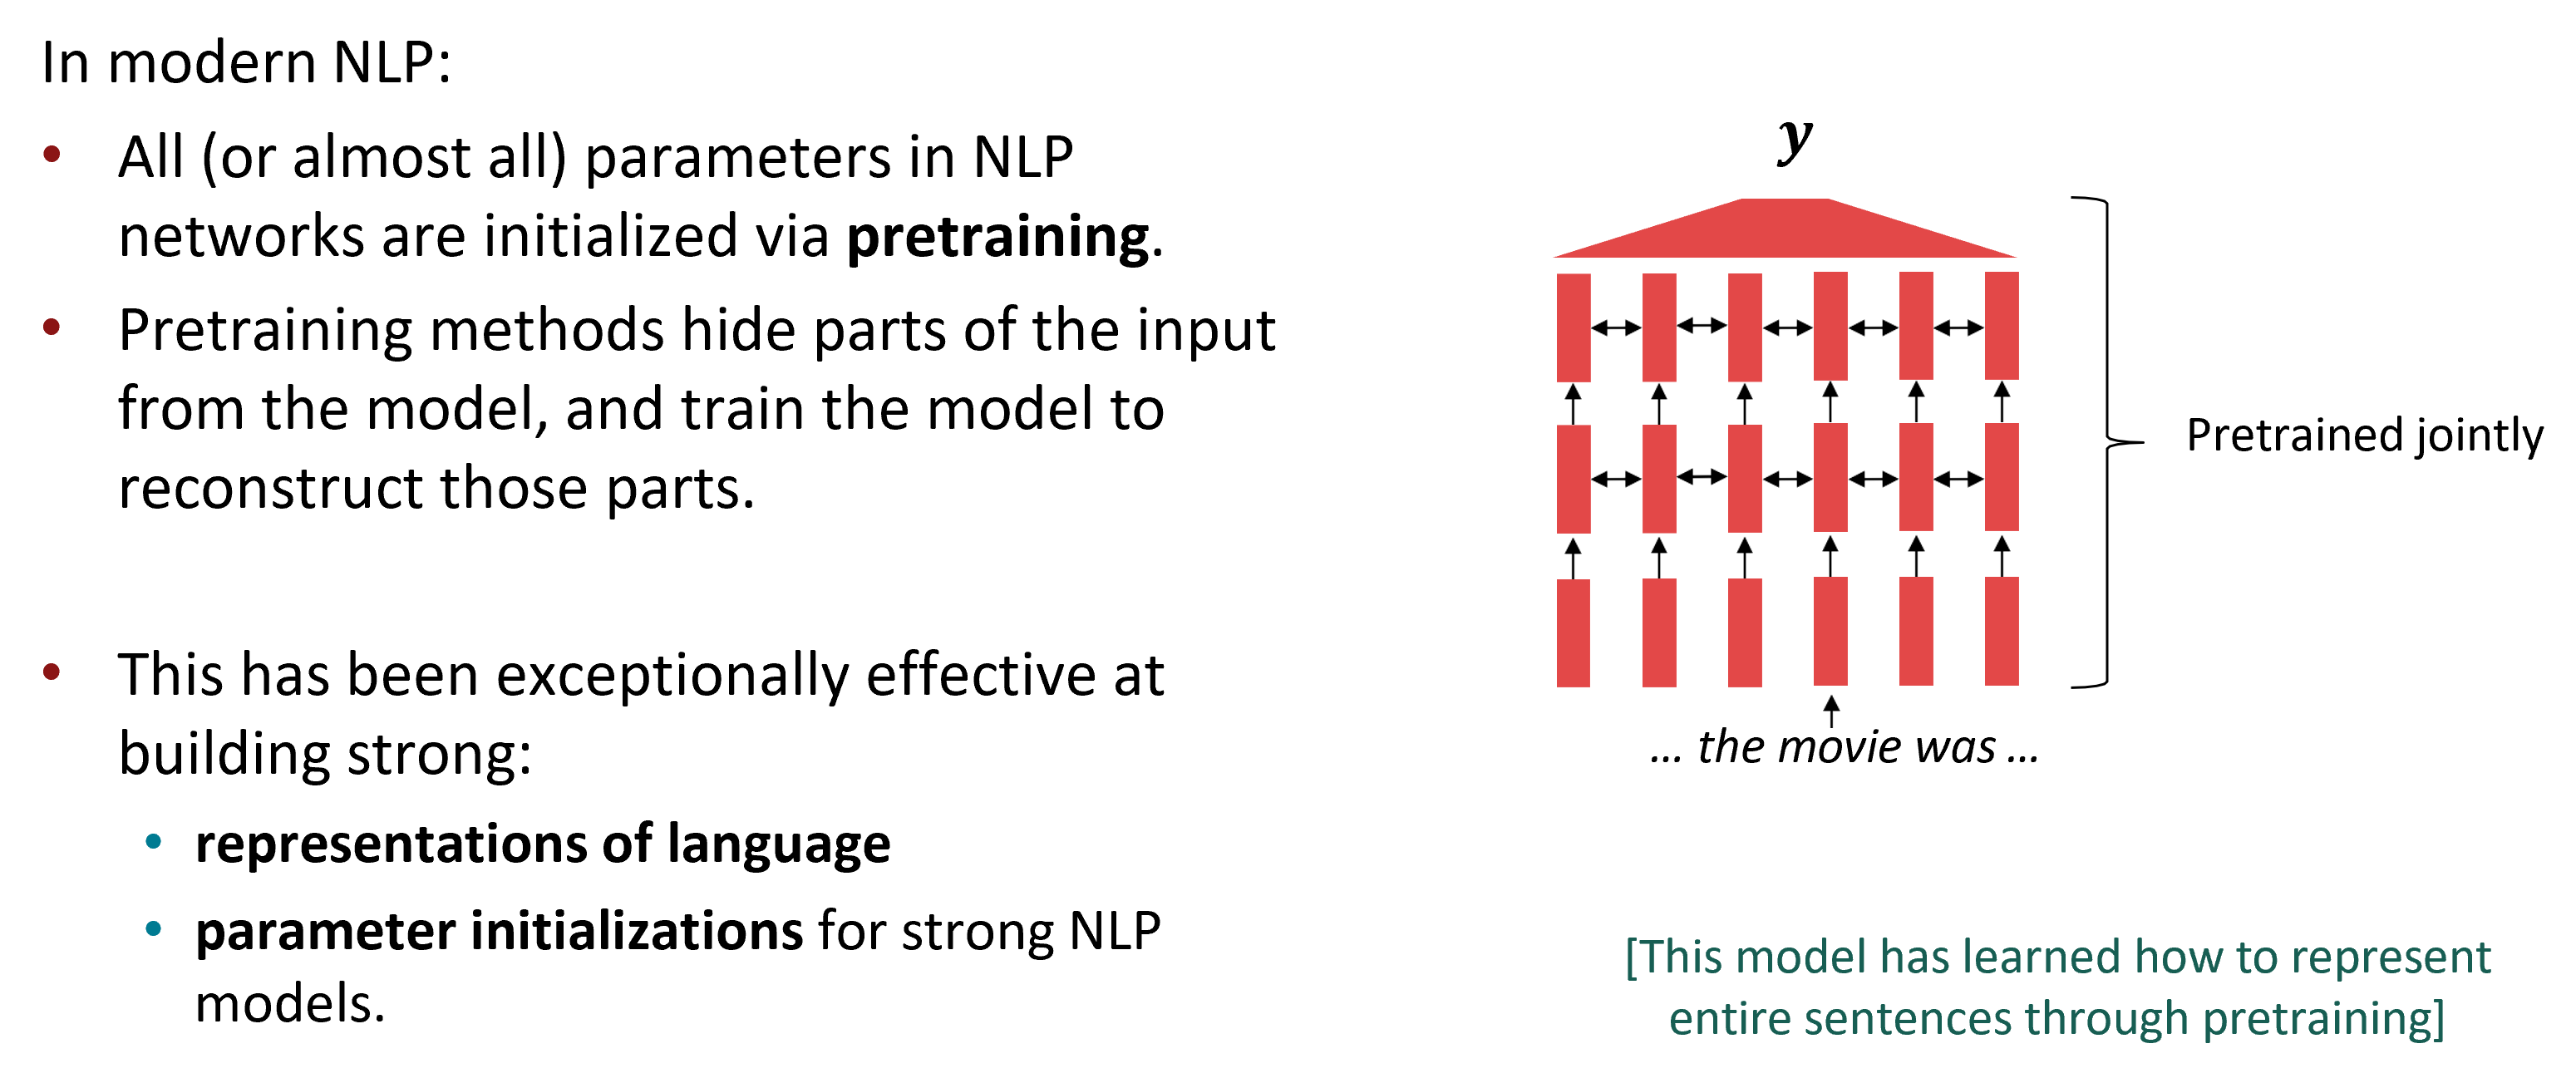
\includegraphics[width=\linewidth,keepaspectratio]{bert96}
			\end{center}		
			
			% {\tiny (Ref: John Hewitt)}

\end{frame}

%%%%%%%%%%%%%%%%%%%%%%%%%%%%%%%%%%%%%%%%%%%%%%%%%%%%%%%%%%%
\begin{frame}[fragile]\frametitle{Pretraining models}
Pretraining through language modeling [Dai and Le, 2015]
			
			\begin{center}
			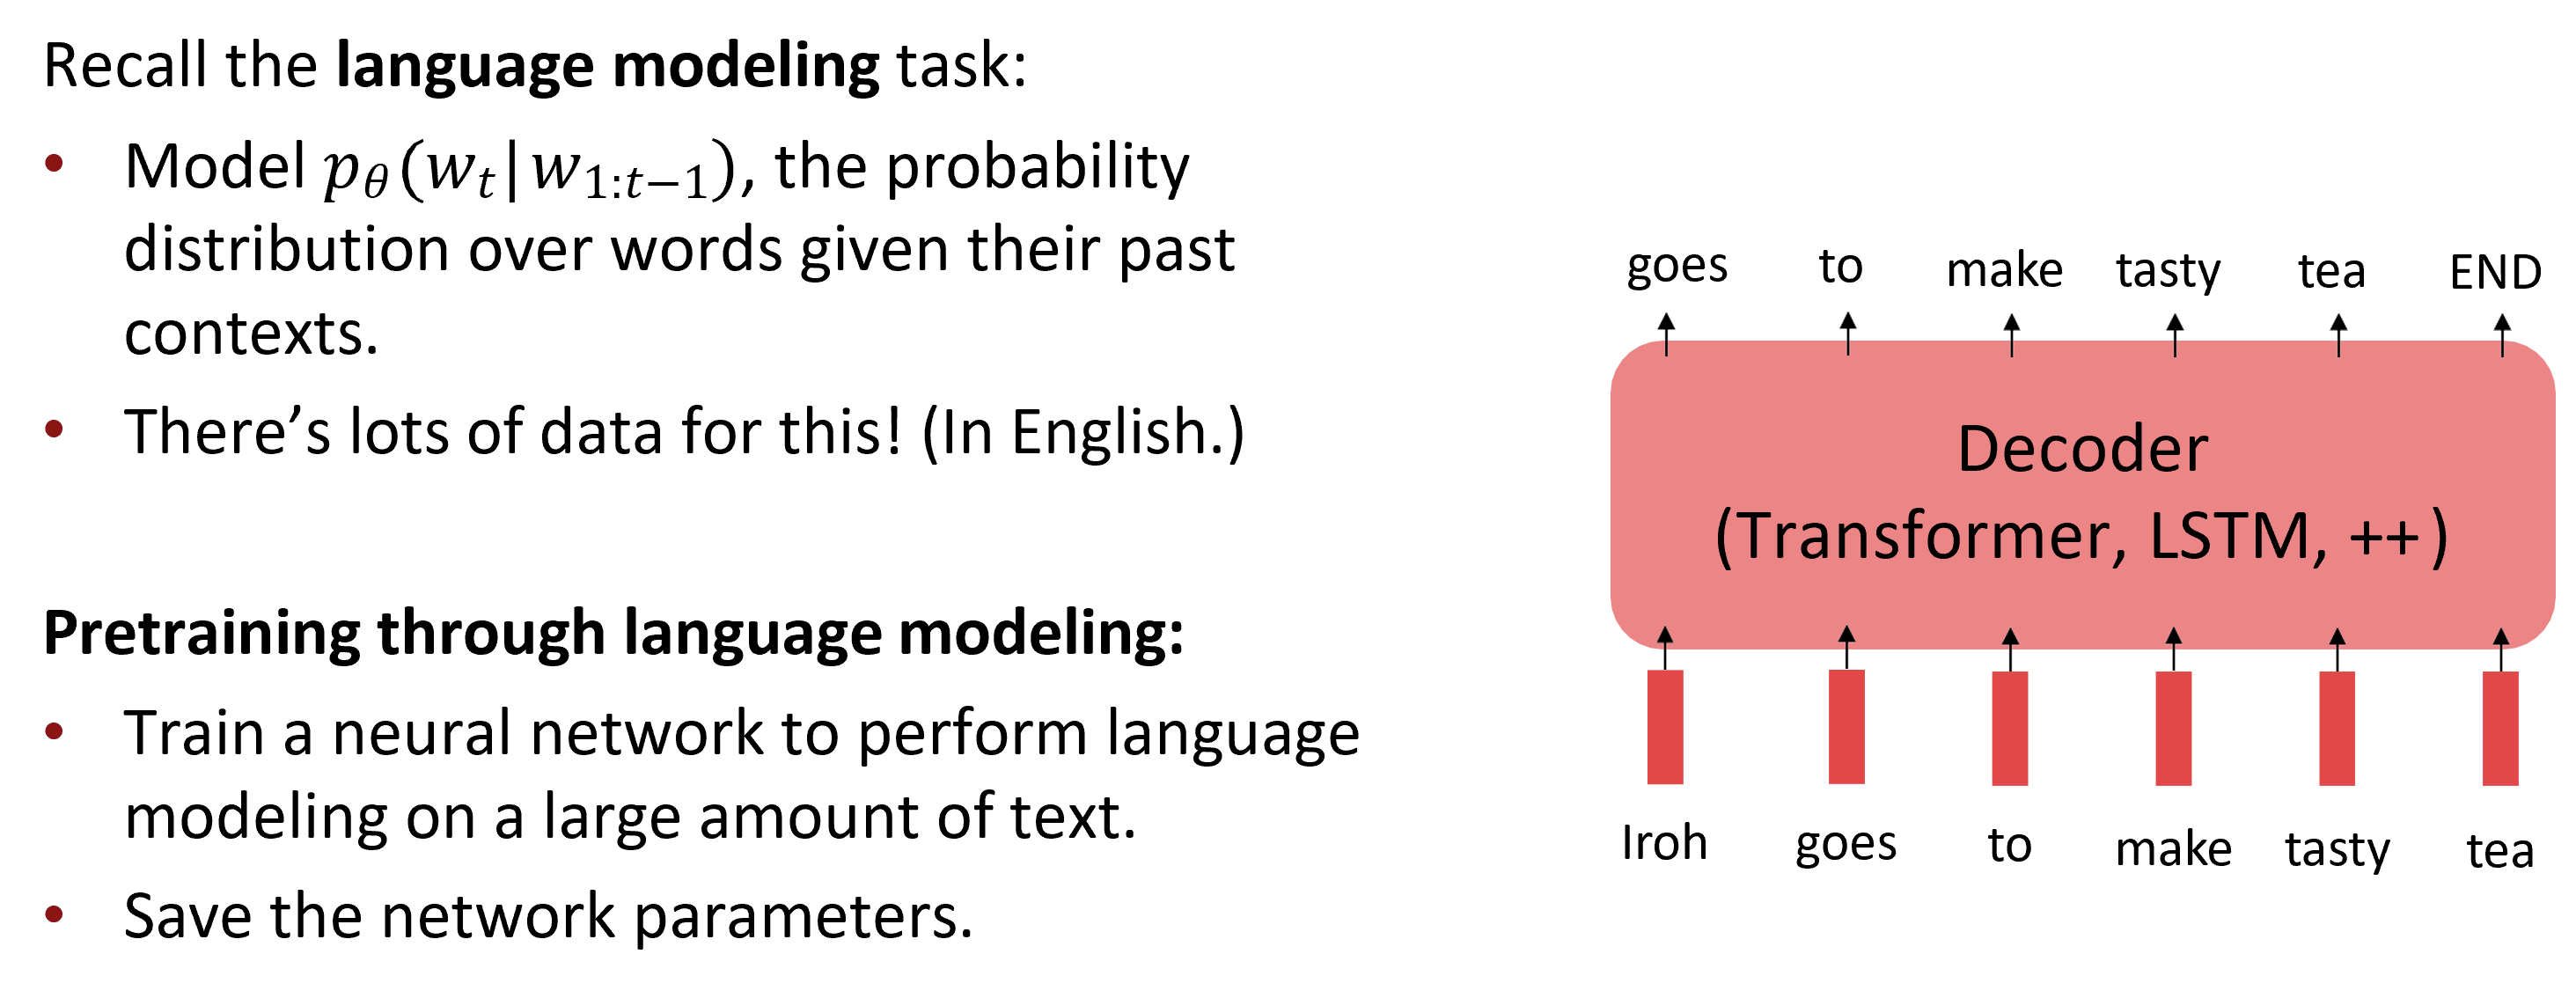
\includegraphics[width=\linewidth,keepaspectratio]{bert97}
			\end{center}		
			
			% {\tiny (Ref: John Hewitt)}

\end{frame}

%%%%%%%%%%%%%%%%%%%%%%%%%%%%%%%%%%%%%%%%%%%%%%%%%%%%%%%%%%%
\begin{frame}[fragile]\frametitle{The Pretraining / Finetuning Paradigm}

			
			\begin{center}
			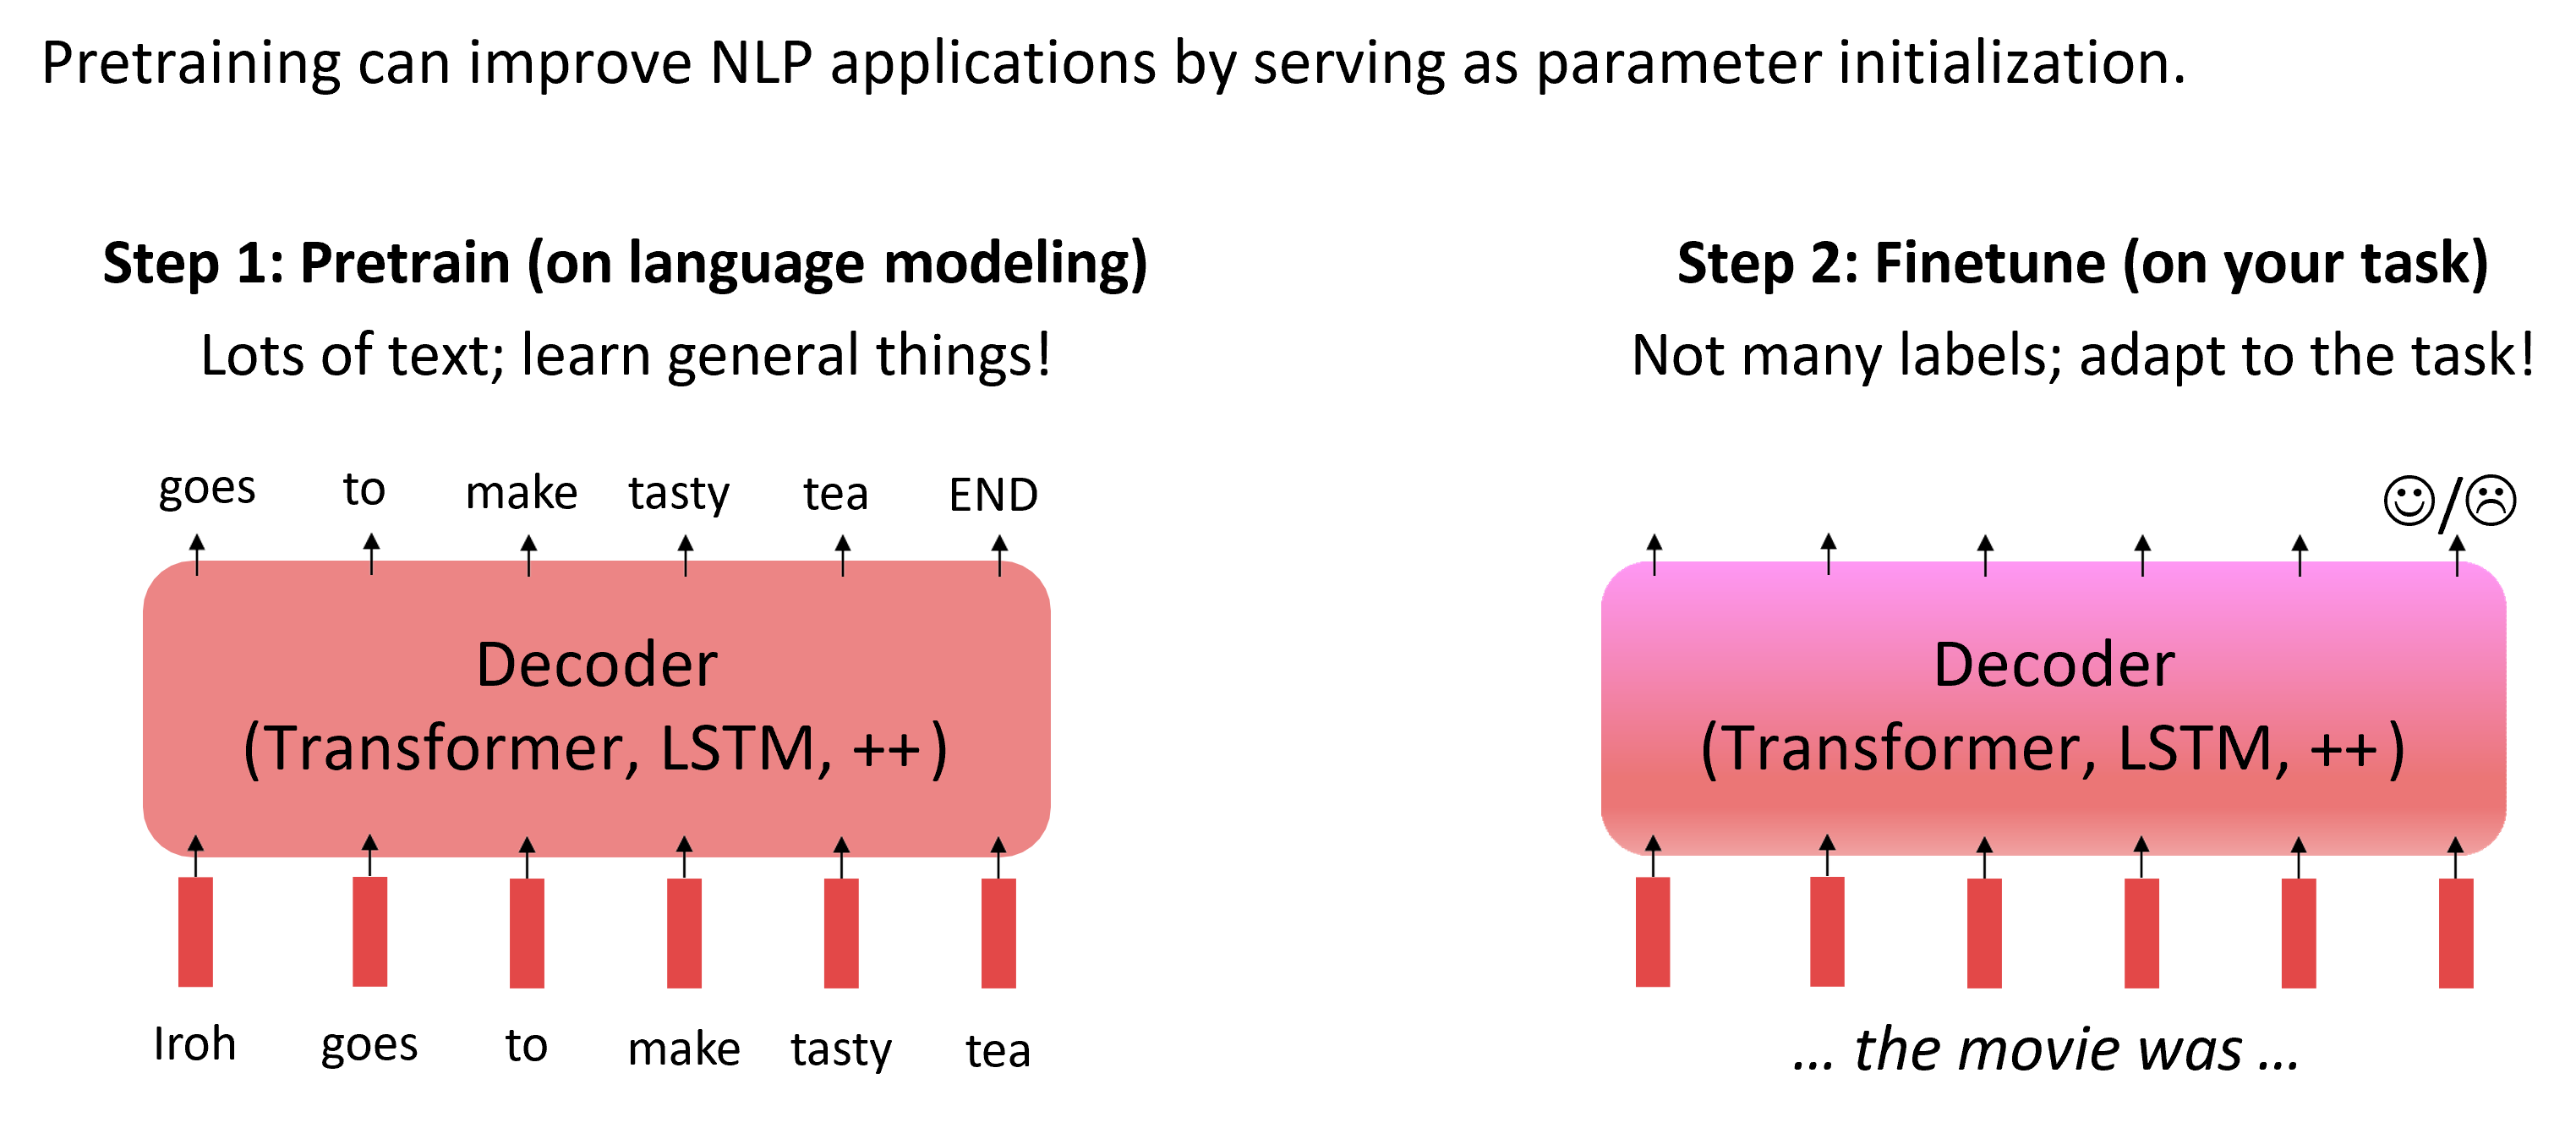
\includegraphics[width=\linewidth,keepaspectratio]{bert98}
			\end{center}		
			
			% {\tiny (Ref: John Hewitt)}

\end{frame}

% %%%%%%%%%%%%%%%%%%%%%%%%%%%%%%%%%%%%%%%%%%%%%%%%%%%%%%%%%%%
% \begin{frame}[fragile]\frametitle{Capturing meaning via context}

% Increasing evidence that pretrained models learn a wide variety of things about
% the statistical properties of language:

      % \begin{itemize}
			% \item Stanford University is located in $--$, California. [Trivia]
			% \item I put $--$ fork down on the table. [syntax]
			% \item The woman walked across the street, checking for traffic over $--$ shoulder. [coreference]
			% \item I went to the ocean to see the fish, turtles, seals, and $--$.	[lexical semantics/topic]
			% \item Overall, the value I got from the two hours watching it was the sum total of the popcorn and the drink. The movie was $--$. [sentiment]
			% \item Iroh went into the kitchen to make some tea. Standing next to Iroh, Zuko pondered his  destiny. Zuko left the $--$. [some reasoning – this is harder]
			% \item I was thinking about the sequence that goes 1, 1, 2, 3, 5, 8, 13, 21, $--$[some basic arithmetic; they don’t learn the Fibonnaci sequence]
			% \item Models also learn – and can exacerbate racism, sexism, all manner of bad biases.
			% \item More on all this in the Interpretability lecture!

			% \end{itemize}

			% % {\tiny (Ref: John Hewitt)}

% \end{frame}

%%%%%%%%%%%%%%%%%%%%%%%%%%%%%%%%%%%%%%%%%%%%%%%%%%%%%%%%%%%
\begin{frame}[fragile]\frametitle{Pretraining}

			Pretraining for three types of architectures
			
			\begin{center}
			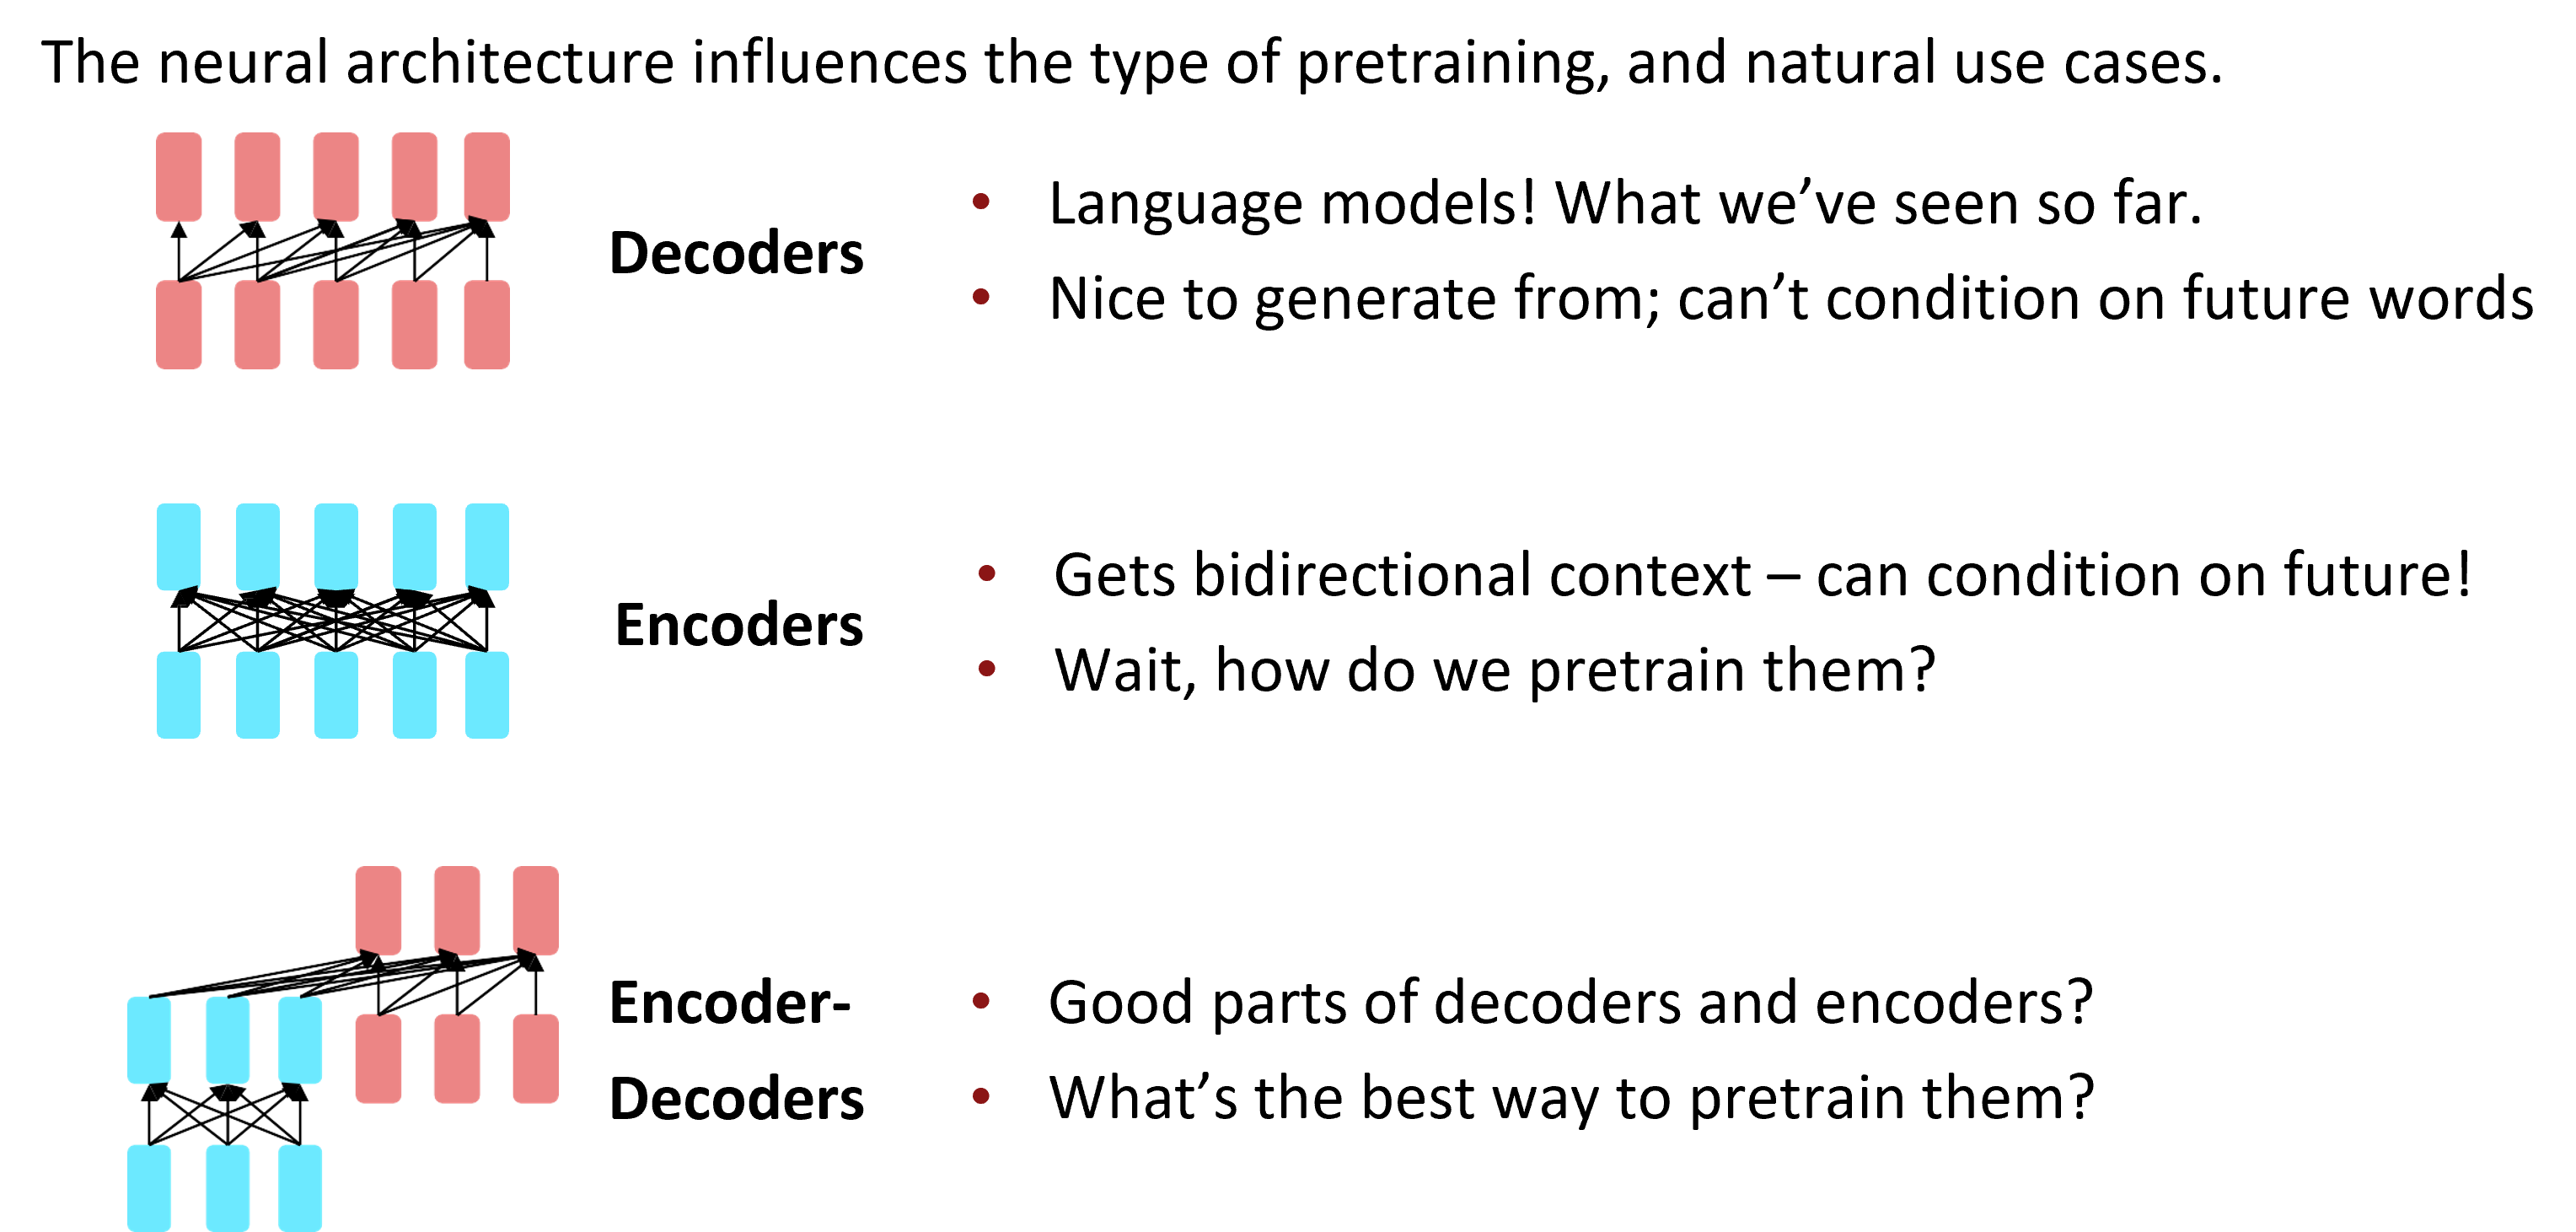
\includegraphics[width=\linewidth,keepaspectratio]{bert99}
			\end{center}		
			
			% {\tiny (Ref: John Hewitt)}

\end{frame}

%%%%%%%%%%%%%%%%%%%%%%%%%%%%%%%%%%%%%%%%%%%%%%%%%%%%%%%%%%%
\begin{frame}[fragile]\frametitle{Pretraining}

			Pretraining encoder-decoders: What pretraining objective to use?
			
			\begin{center}
			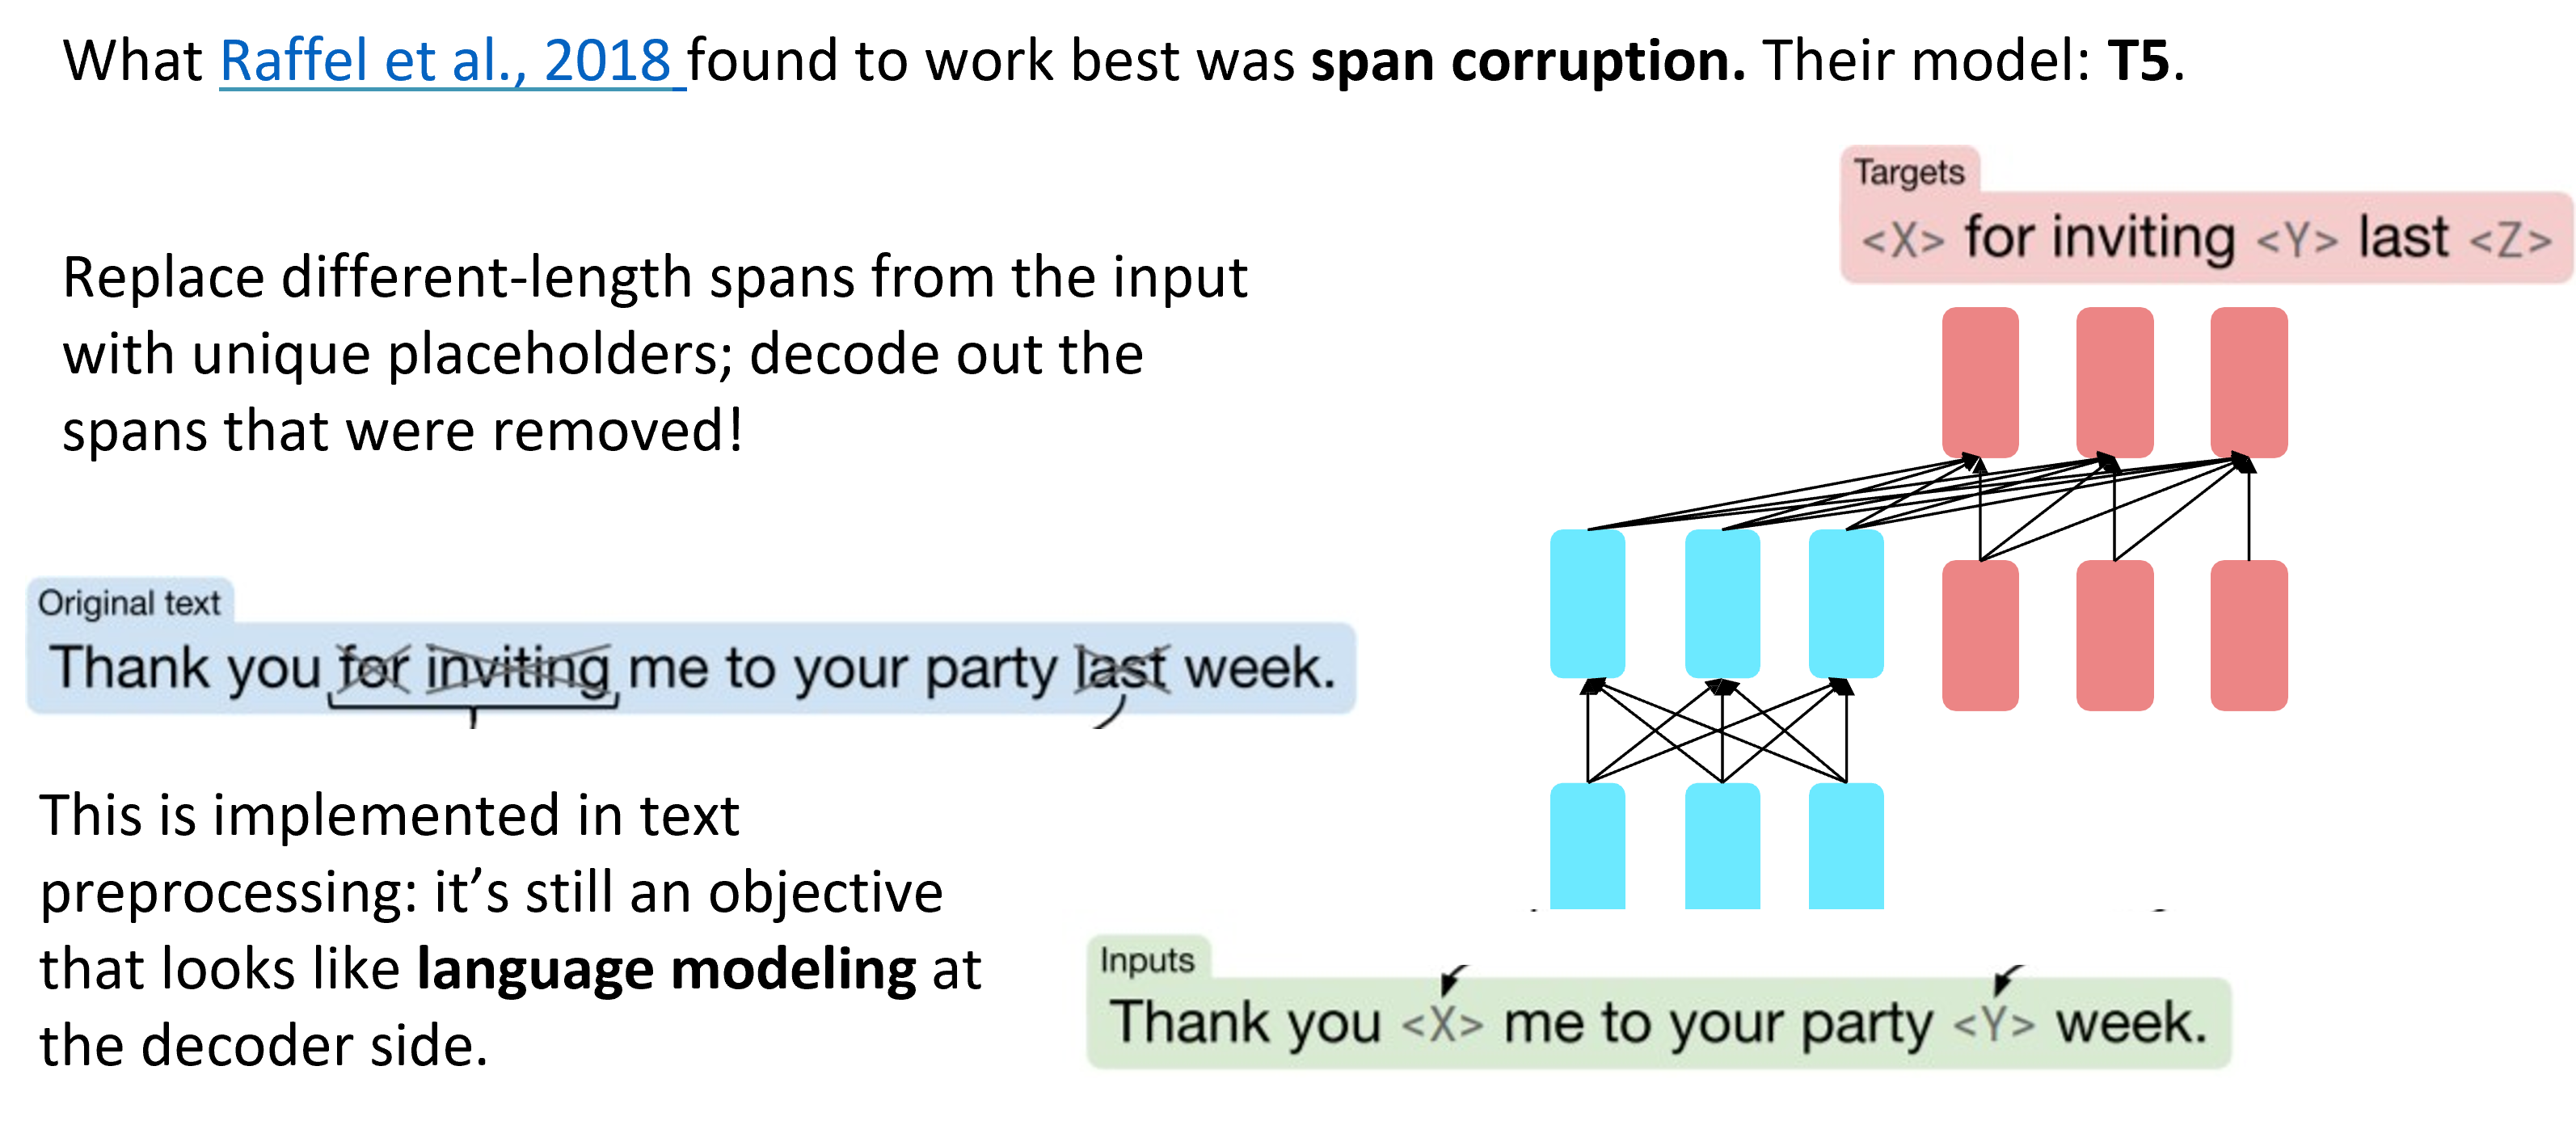
\includegraphics[width=\linewidth,keepaspectratio]{bert100}
			\end{center}		
			
			% {\tiny (Ref: John Hewitt)}

\end{frame}

%%%%%%%%%%%%%%%%%%%%%%%%%%%%%%%%%%%%%%%%%%%%%%%%%%%%%%%%%%%
\begin{frame}[fragile]\frametitle{Pretraining}

			Pretraining encoder-decoders: What pretraining objective to use?

			
			\begin{center}
			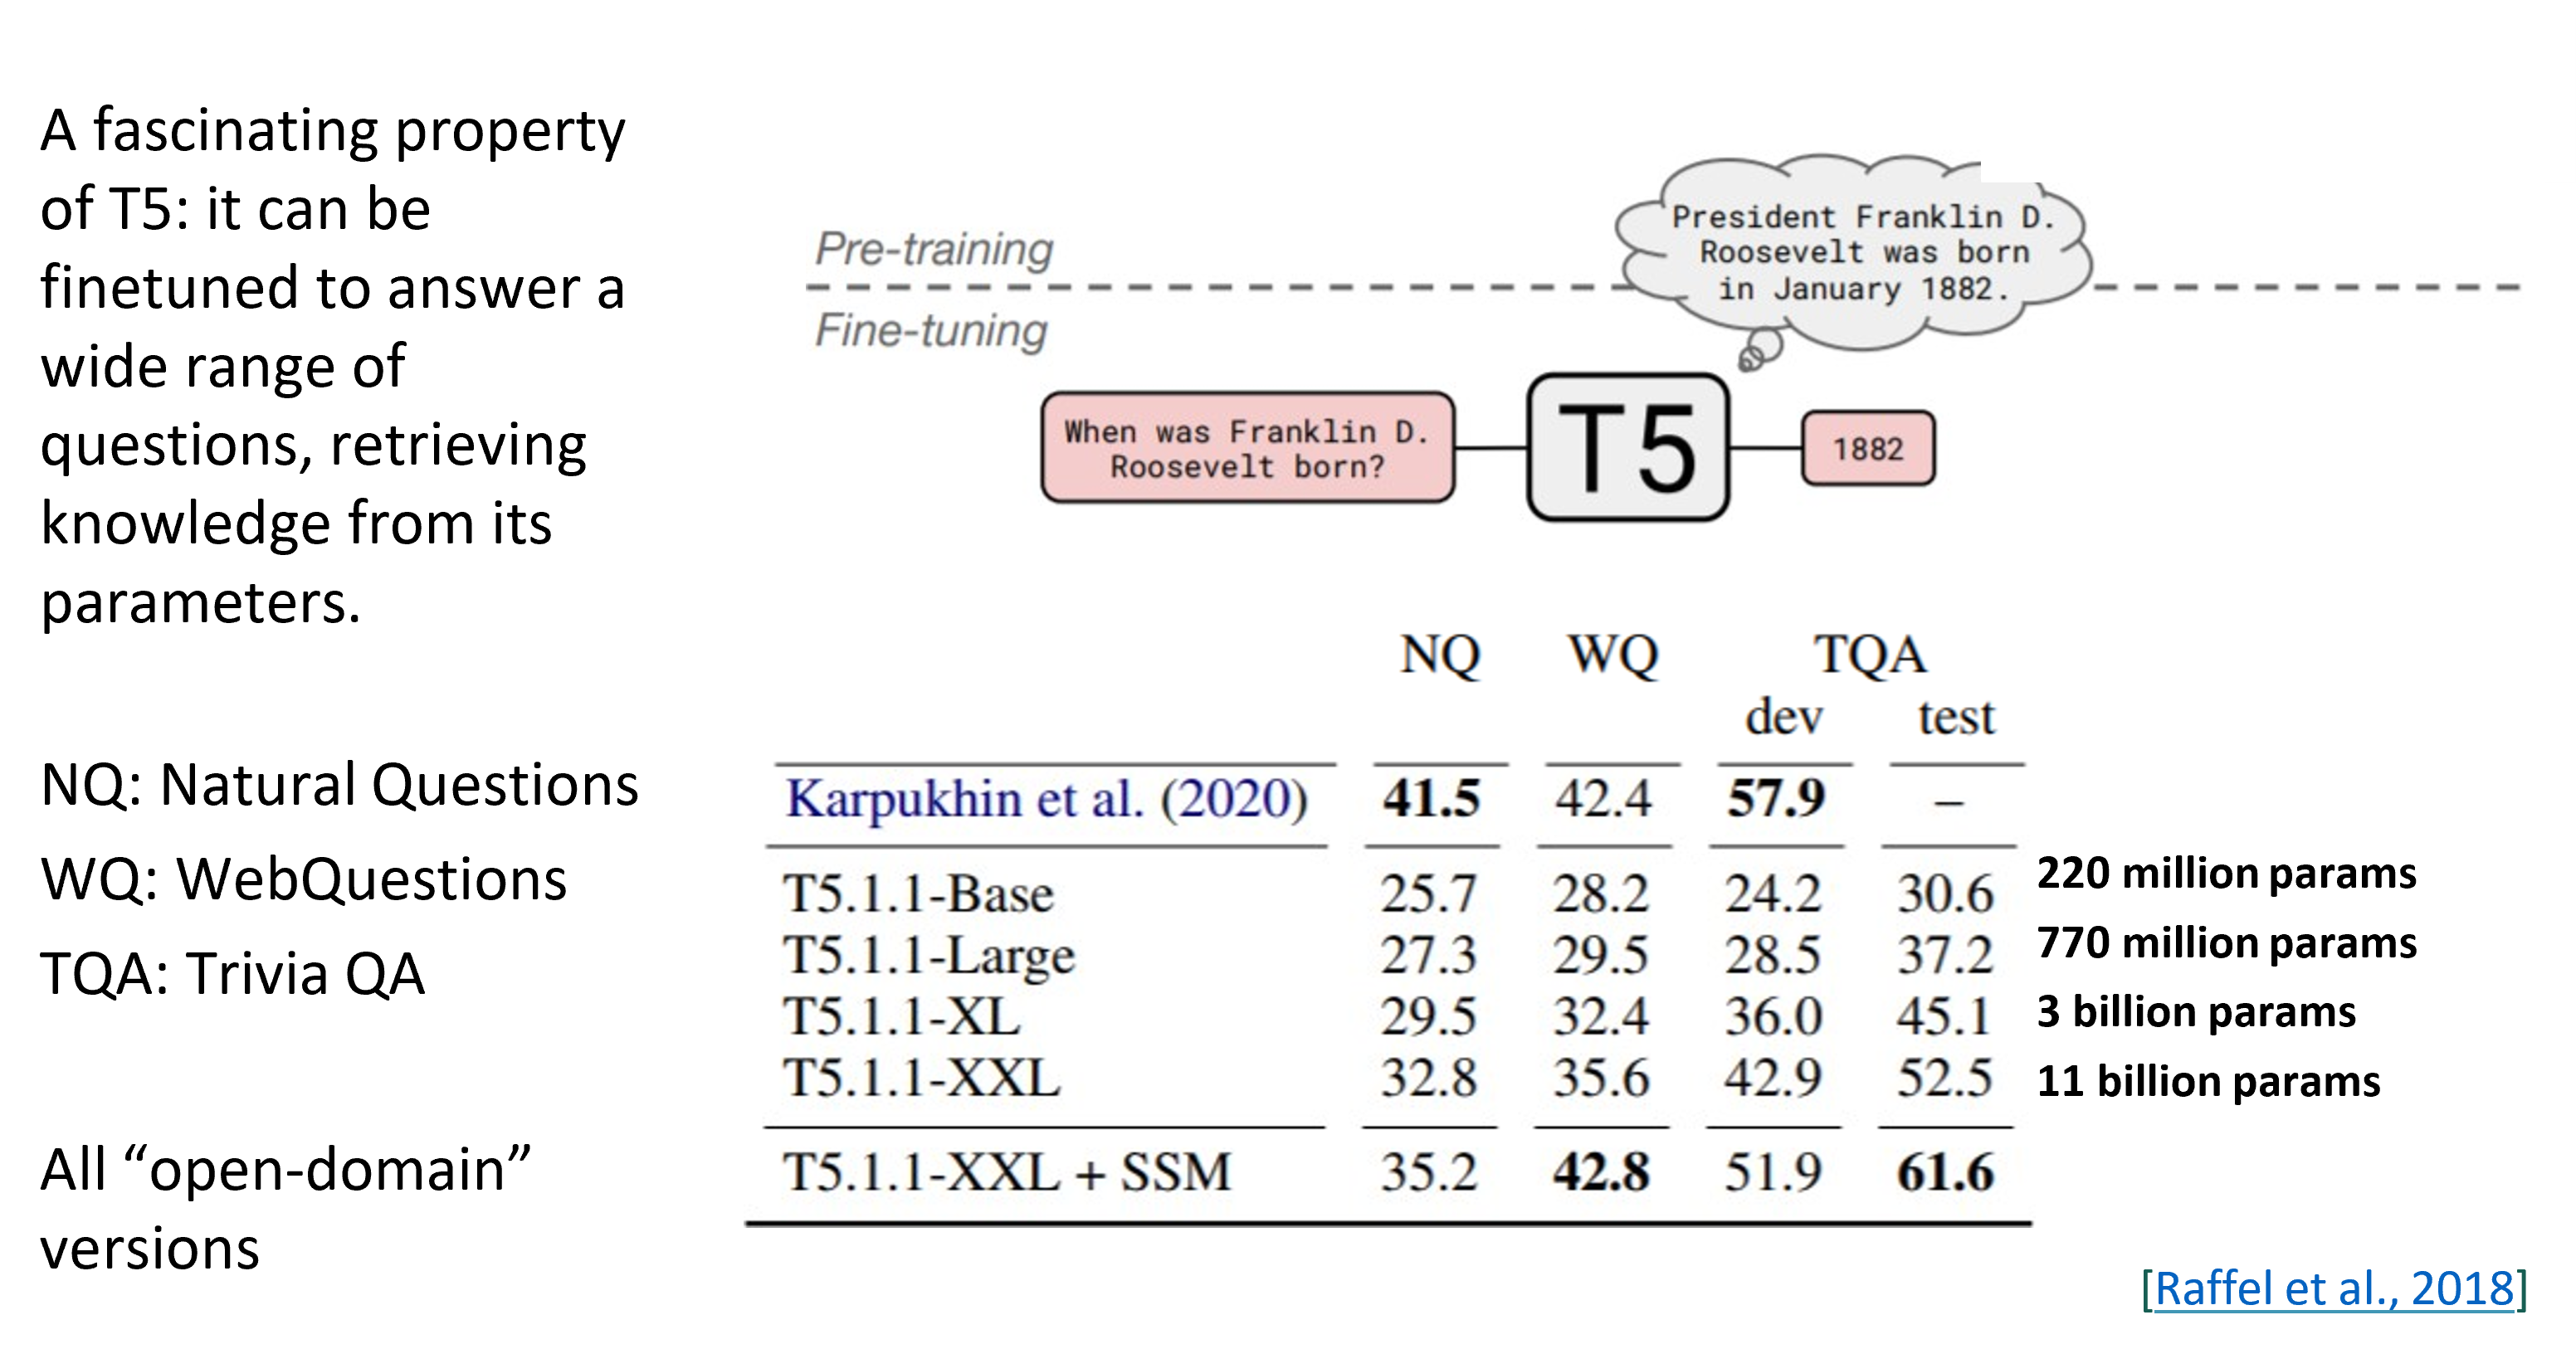
\includegraphics[width=\linewidth,keepaspectratio]{bert101}
			\end{center}		
			
			% {\tiny (Ref: John Hewitt)}

\end{frame}


%%%%%%%%%%%%%%%%%%%%%%%%%%%%%%%%%%%%%%%%%%%%%%%%%%%%%%%%%%%
\begin{frame}[fragile]\frametitle{Pretraining decoders}


			\begin{center}
			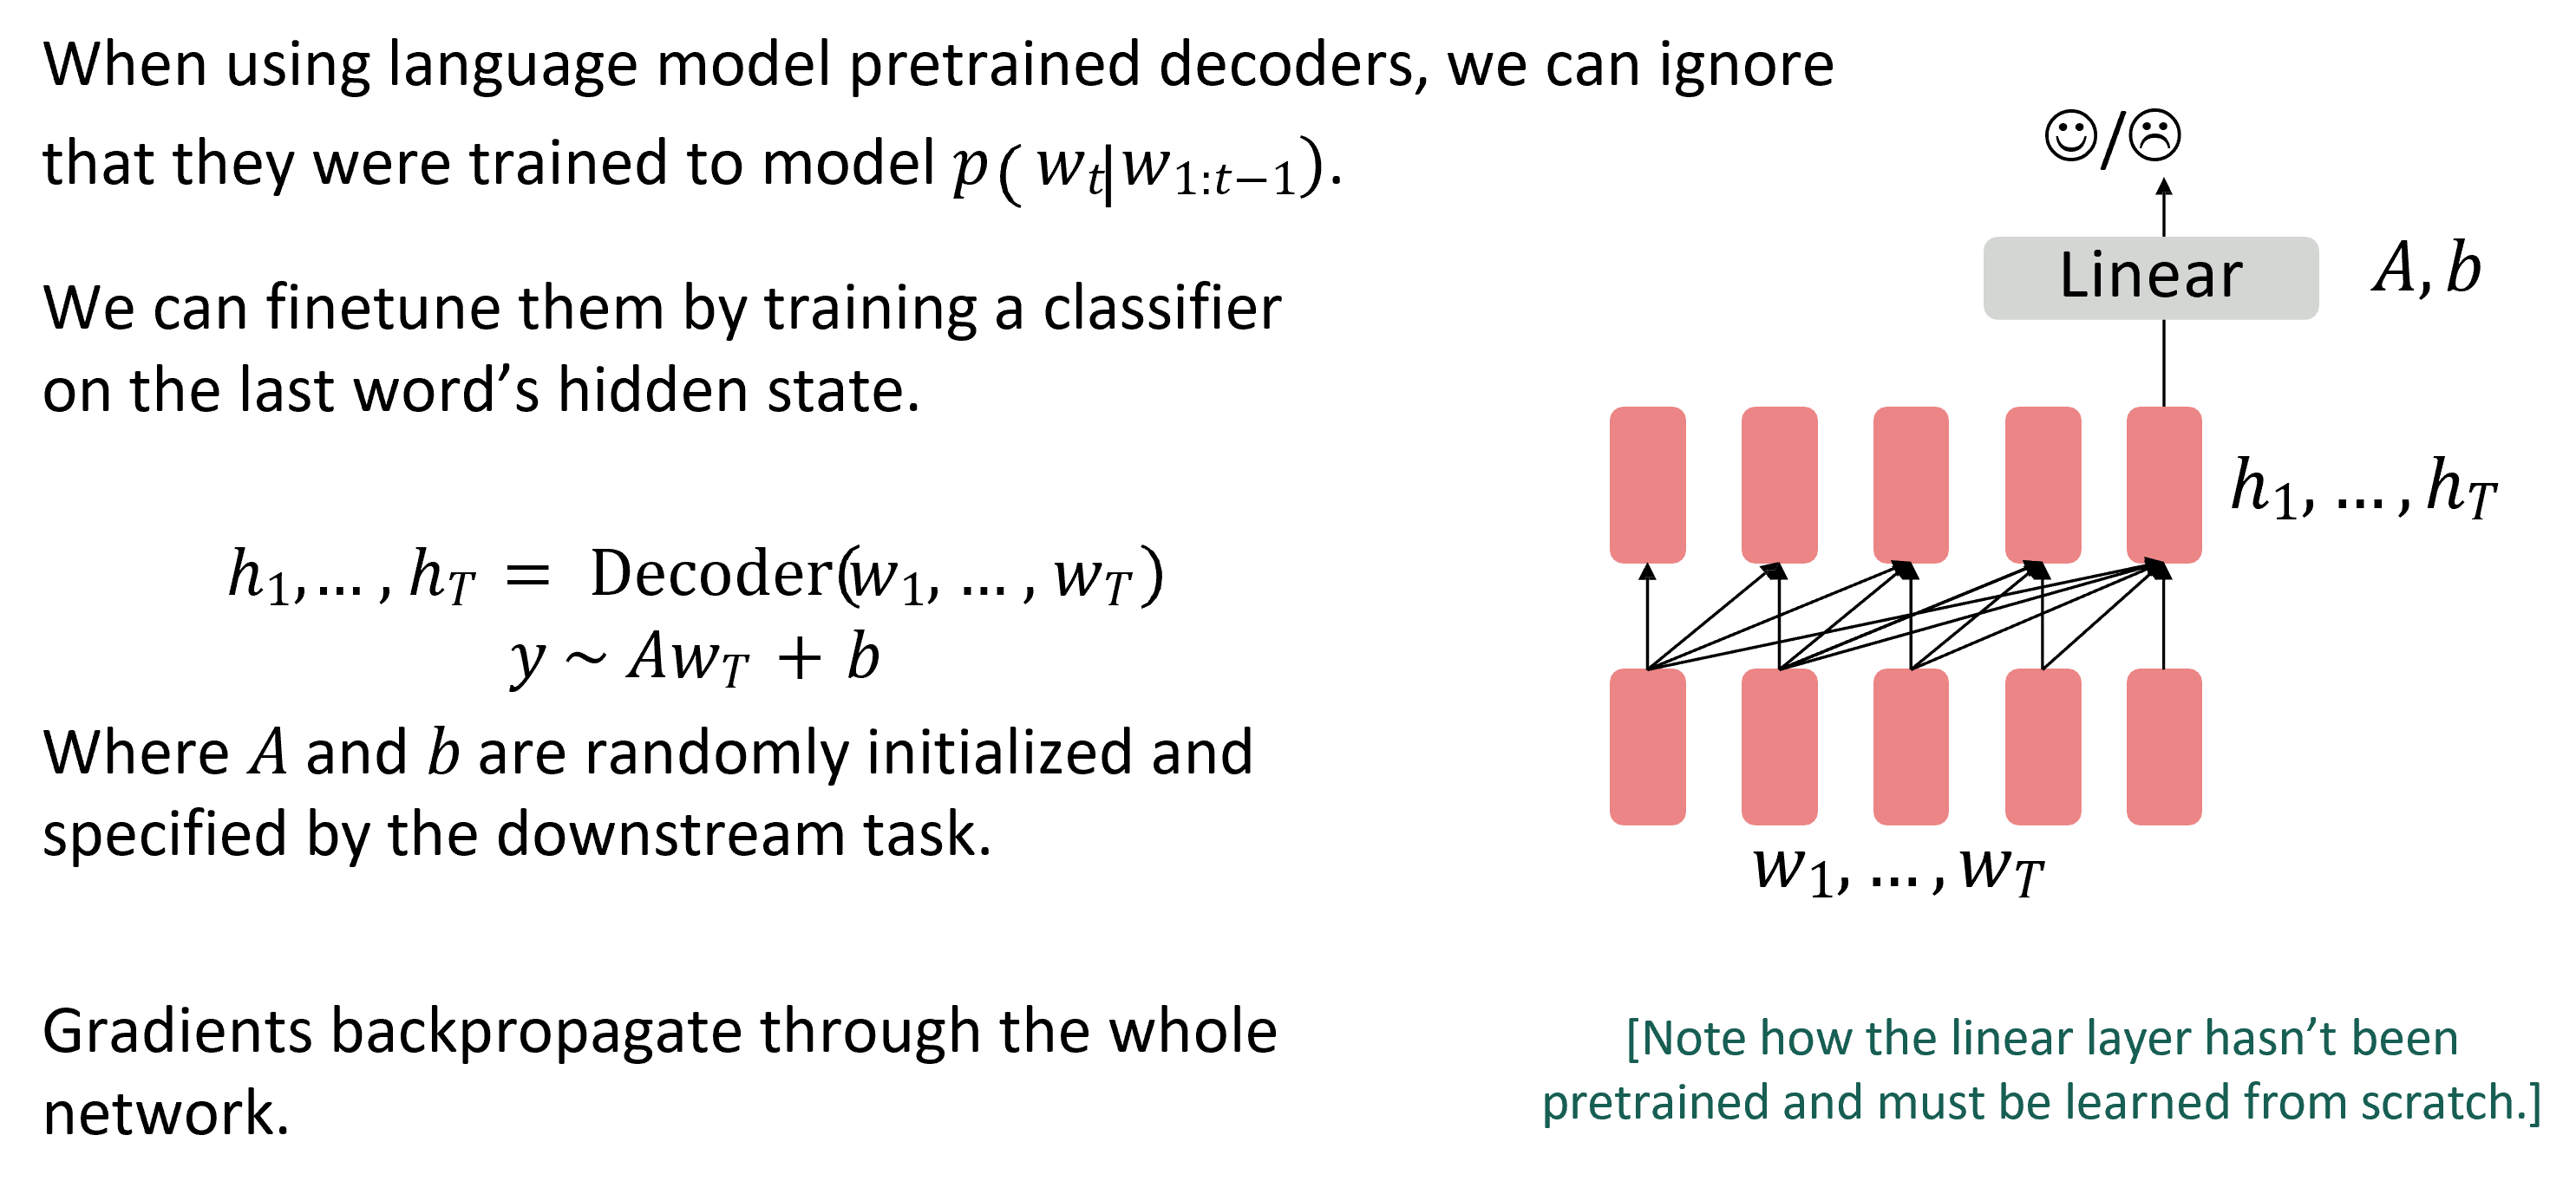
\includegraphics[width=\linewidth,keepaspectratio]{bert104}
			\end{center}		
			
			% {\tiny (Ref: John Hewitt)}

\end{frame}

%%%%%%%%%%%%%%%%%%%%%%%%%%%%%%%%%%%%%%%%%%%%%%%%%%%%%%%%%%%
\begin{frame}[fragile]\frametitle{Pretraining decoders}


			\begin{center}
			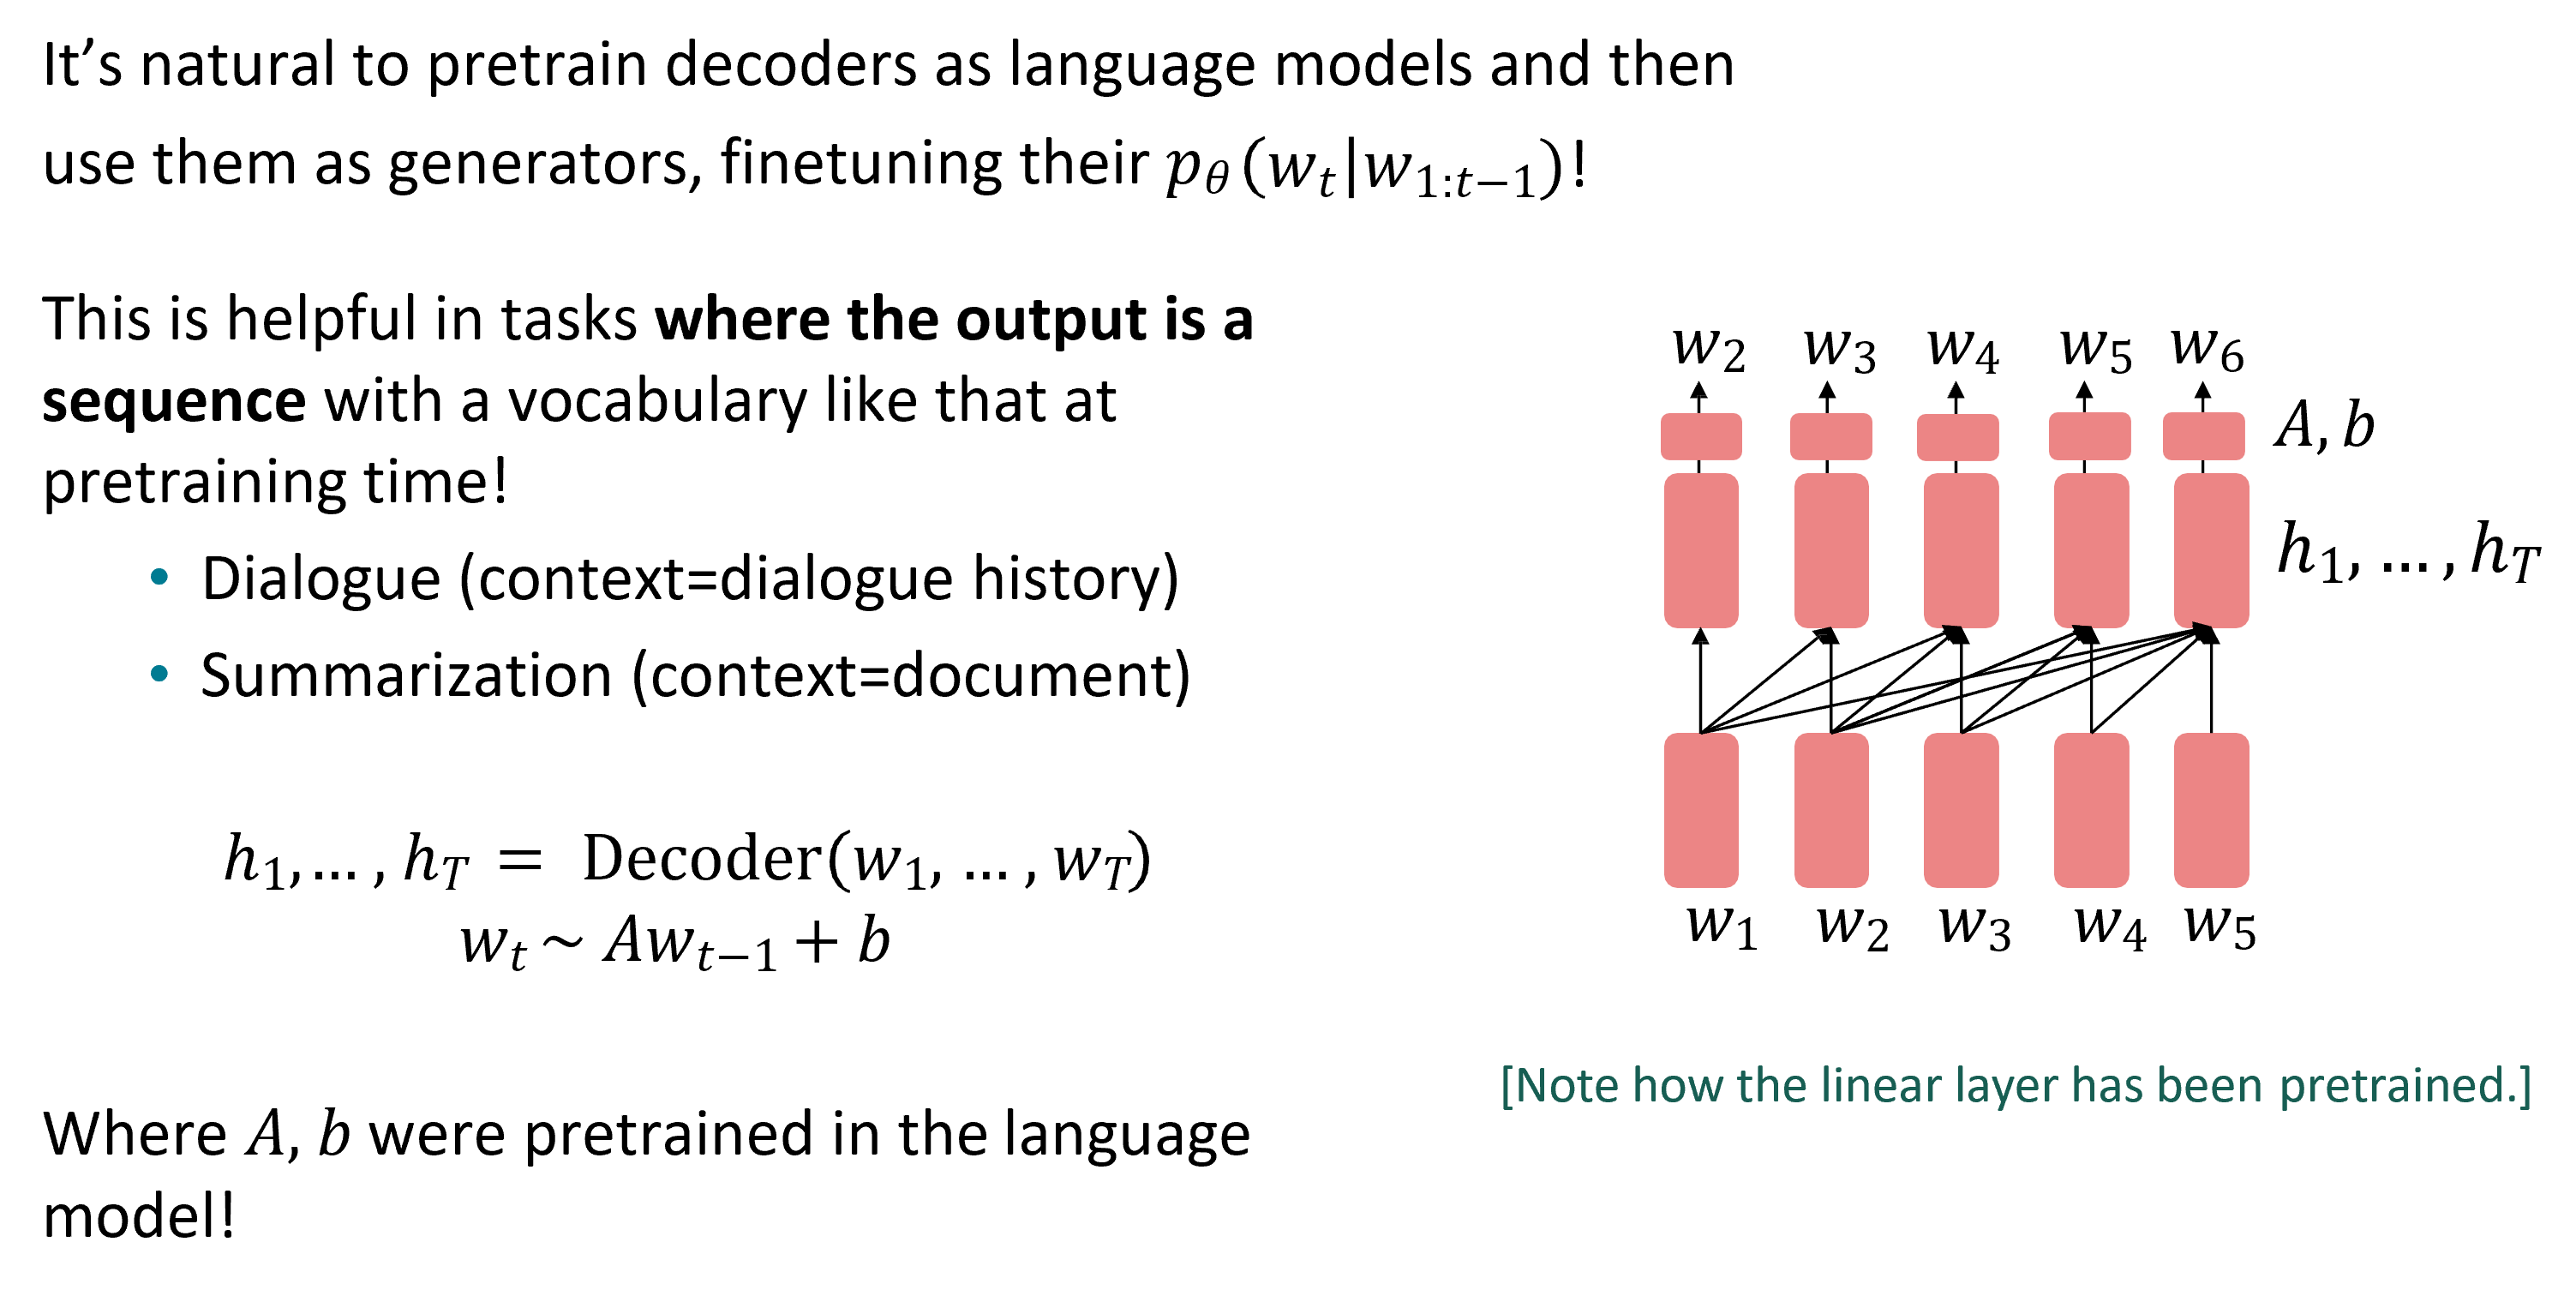
\includegraphics[width=\linewidth,keepaspectratio]{bert105}
			\end{center}		
			
			% {\tiny (Ref: John Hewitt)}

\end{frame}

% %%%%%%%%%%%%%%%%%%%%%%%%%%%%%%%%%%%%%%%%%%%%%%%%%%%%%%%%%%%
% \begin{frame}[fragile]\frametitle{Aside: Word structure and subword models}

			% \begin{center}
			% 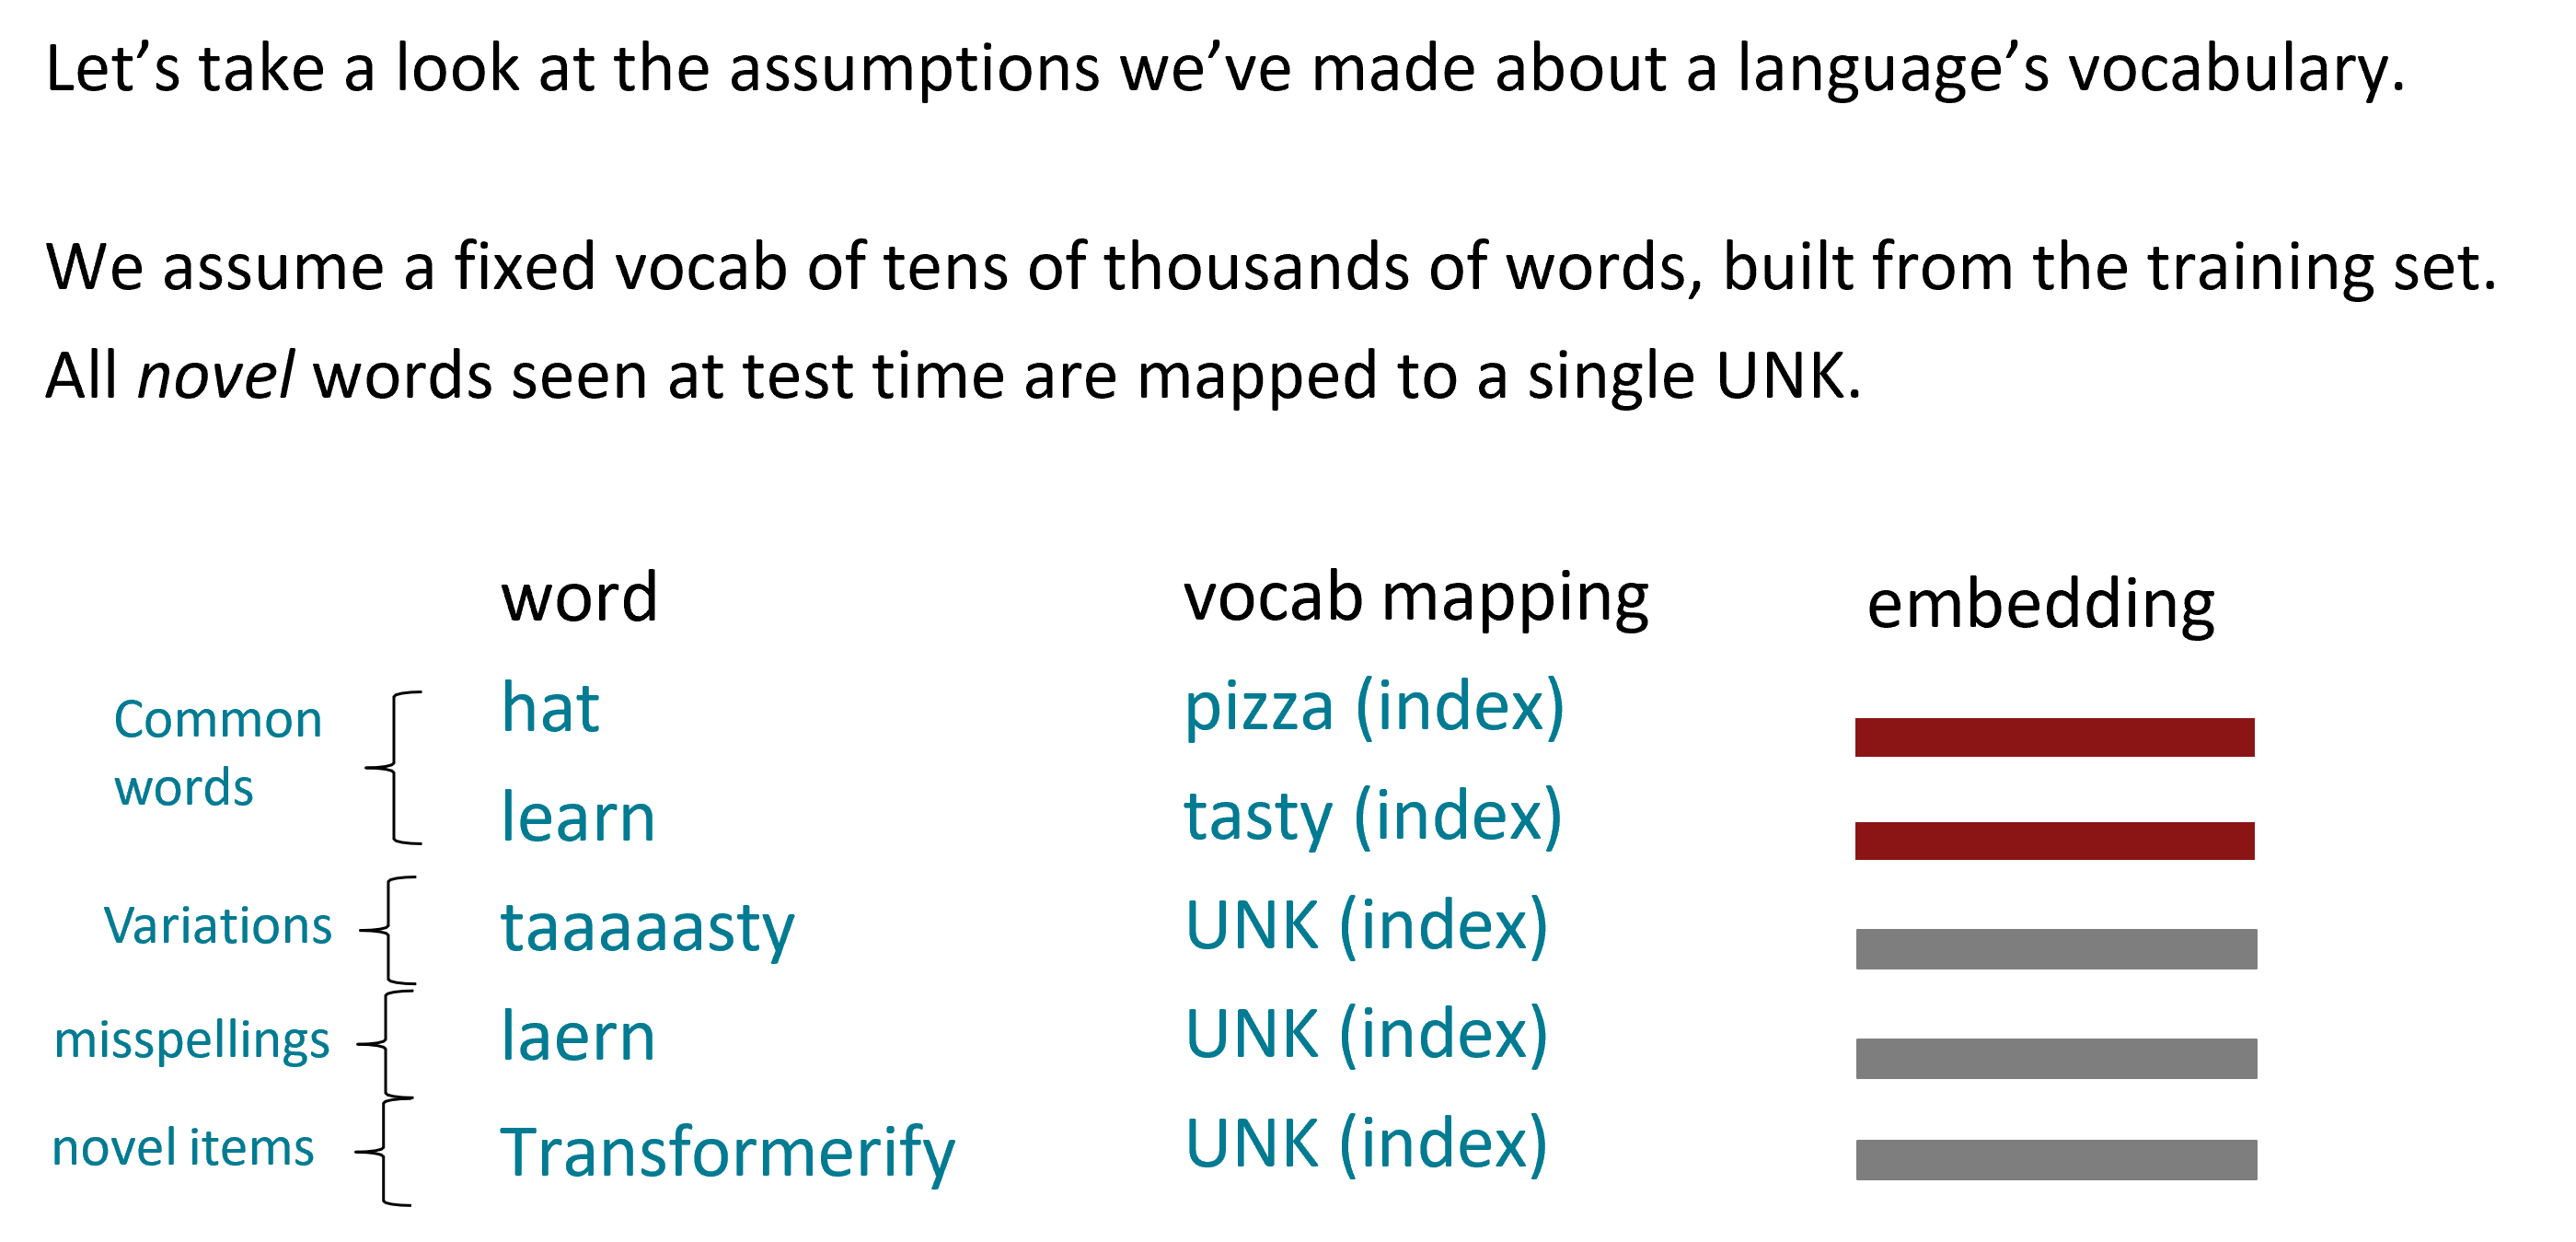
\includegraphics[width=\linewidth,keepaspectratio]{bert109}
			% \end{center}		
			
			% % {\tiny (Ref: John Hewitt)}

% \end{frame}

% %%%%%%%%%%%%%%%%%%%%%%%%%%%%%%%%%%%%%%%%%%%%%%%%%%%%%%%%%%%
% \begin{frame}[fragile]\frametitle{Aside: Word structure and subword models}

			% \begin{center}
			% 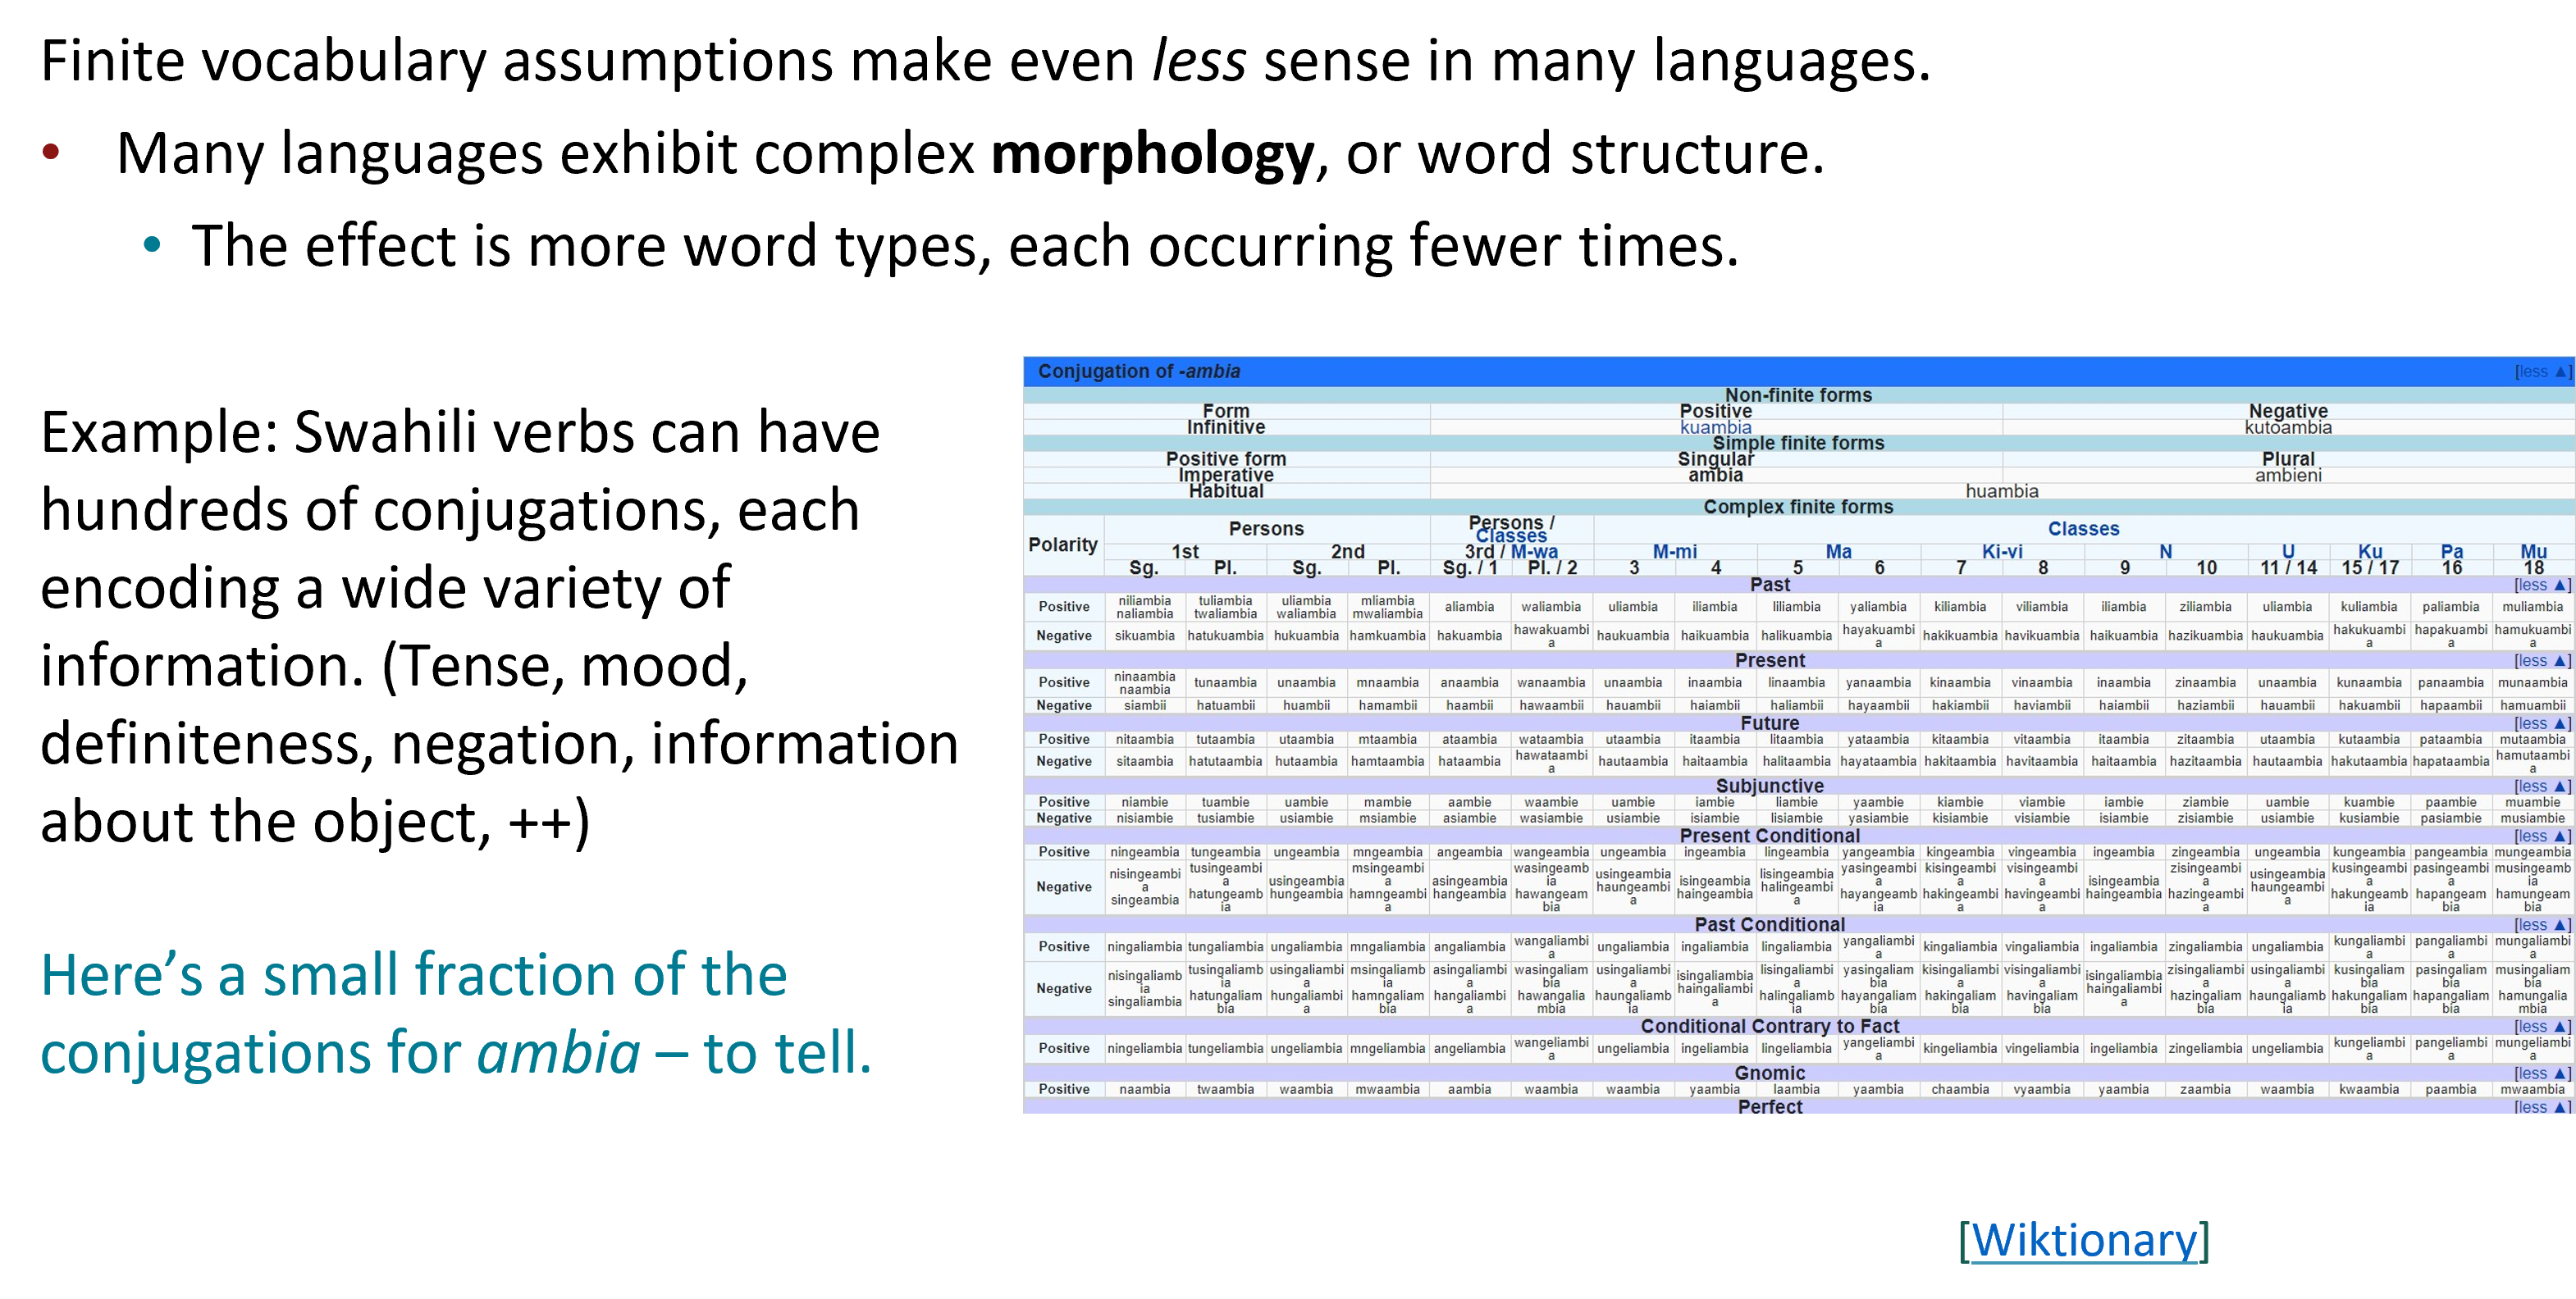
\includegraphics[width=\linewidth,keepaspectratio]{bert110}
			% \end{center}		
			
			% % {\tiny (Ref: John Hewitt)}

% \end{frame}


% %%%%%%%%%%%%%%%%%%%%%%%%%%%%%%%%%%%%%%%%%%%%%%%%%%%%%%%%%%%
% \begin{frame}[fragile]\frametitle{Aside: The byte-pair encoding algorithm}

			% \begin{center}
			% 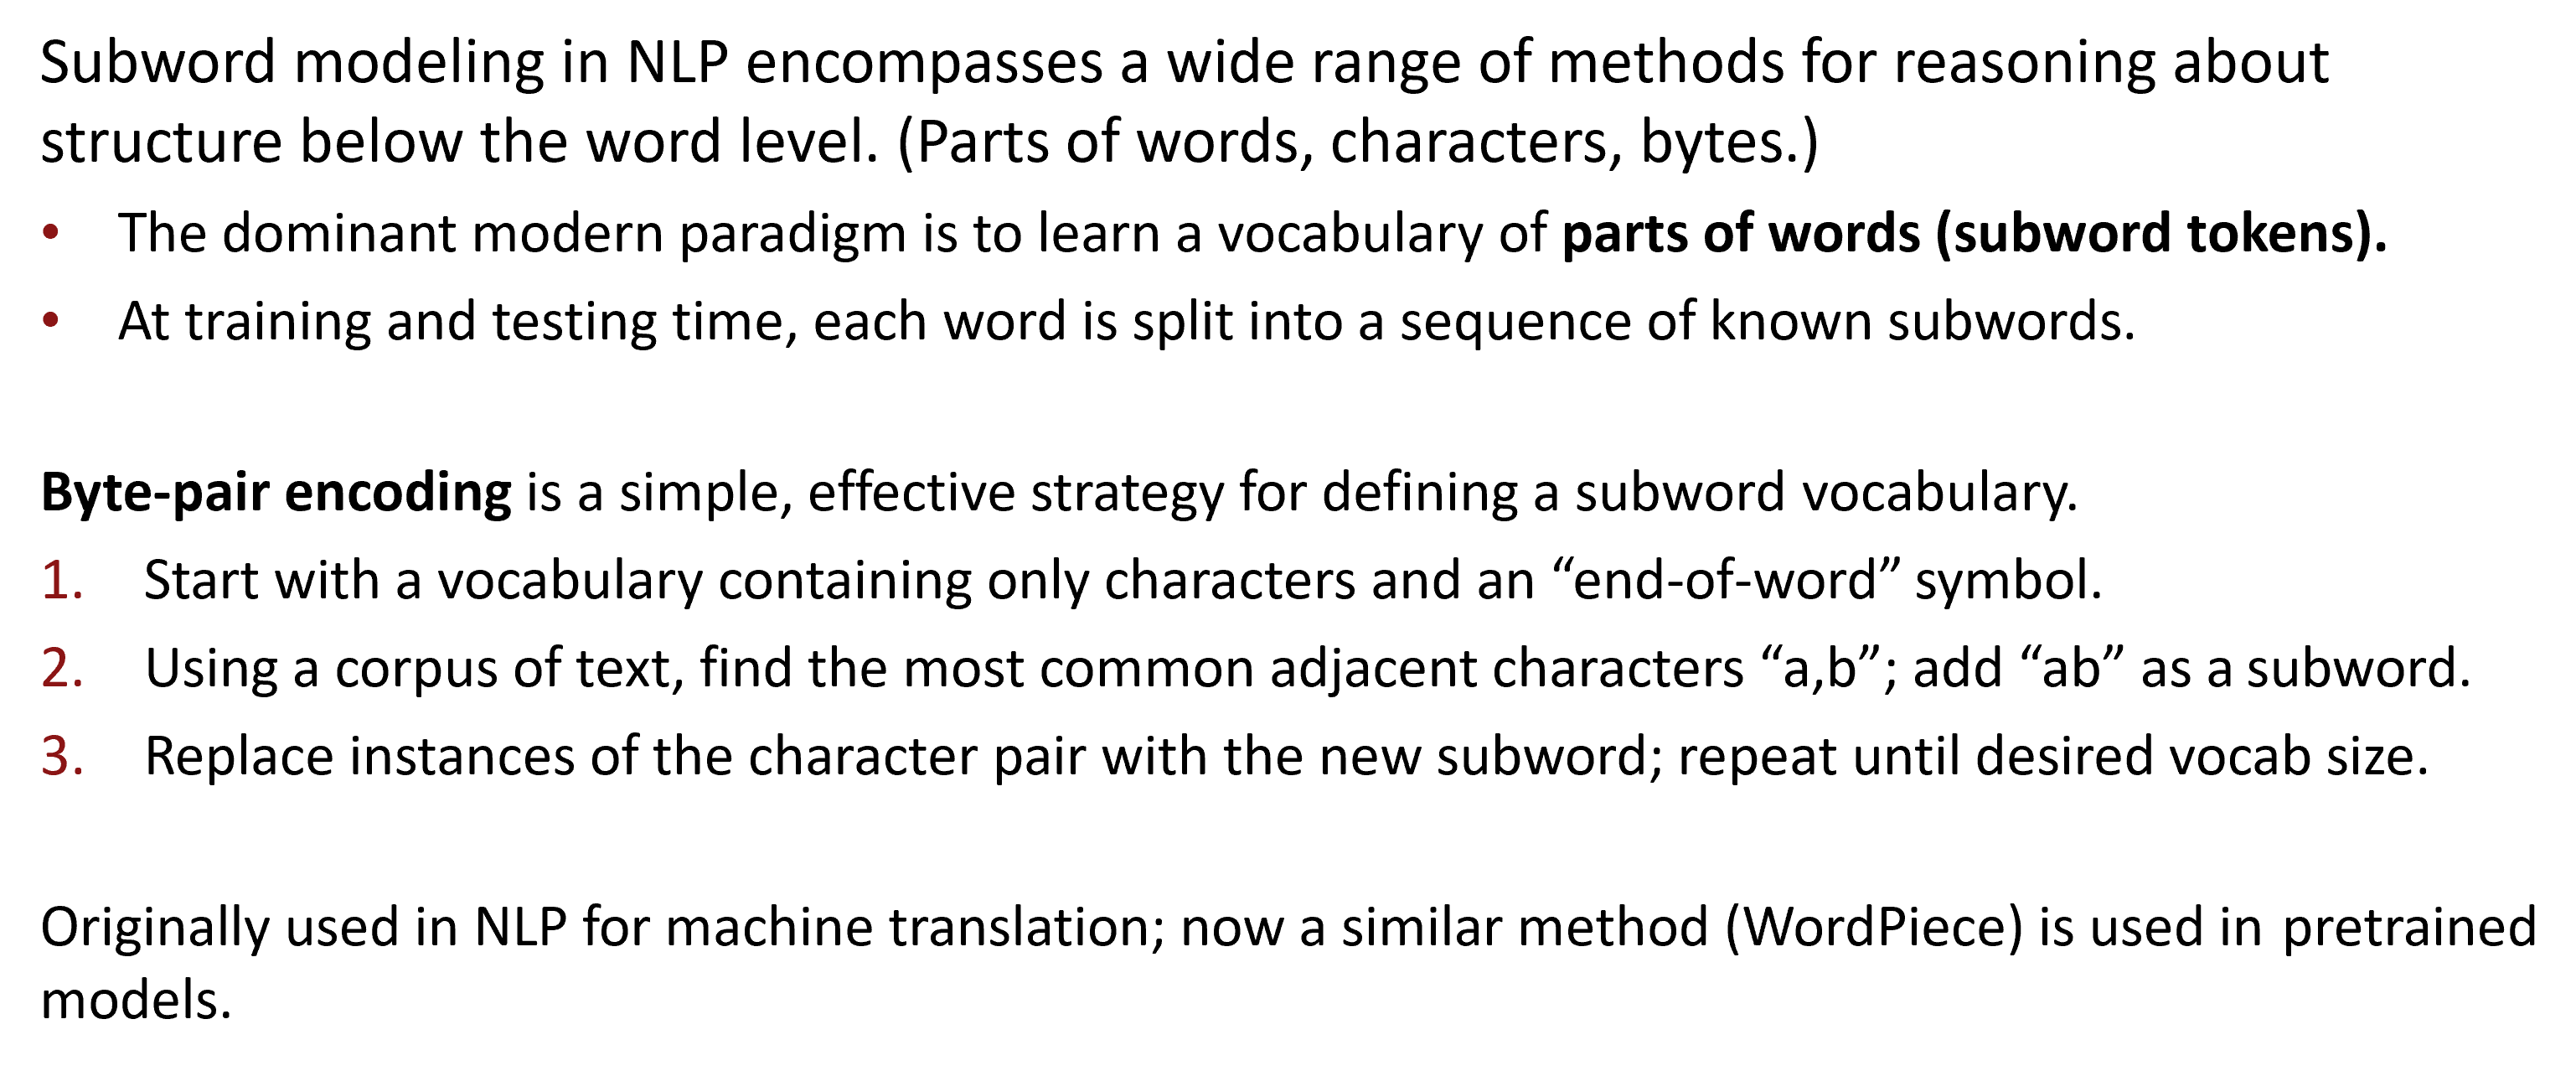
\includegraphics[width=\linewidth,keepaspectratio]{bert111}
			% \end{center}		
			
			% % {\tiny (Ref: John Hewitt)}

% \end{frame}

% %%%%%%%%%%%%%%%%%%%%%%%%%%%%%%%%%%%%%%%%%%%%%%%%%%%%%%%%%%%
% \begin{frame}[fragile]\frametitle{Aside: Word structure and subword models}

			% \begin{center}
			% 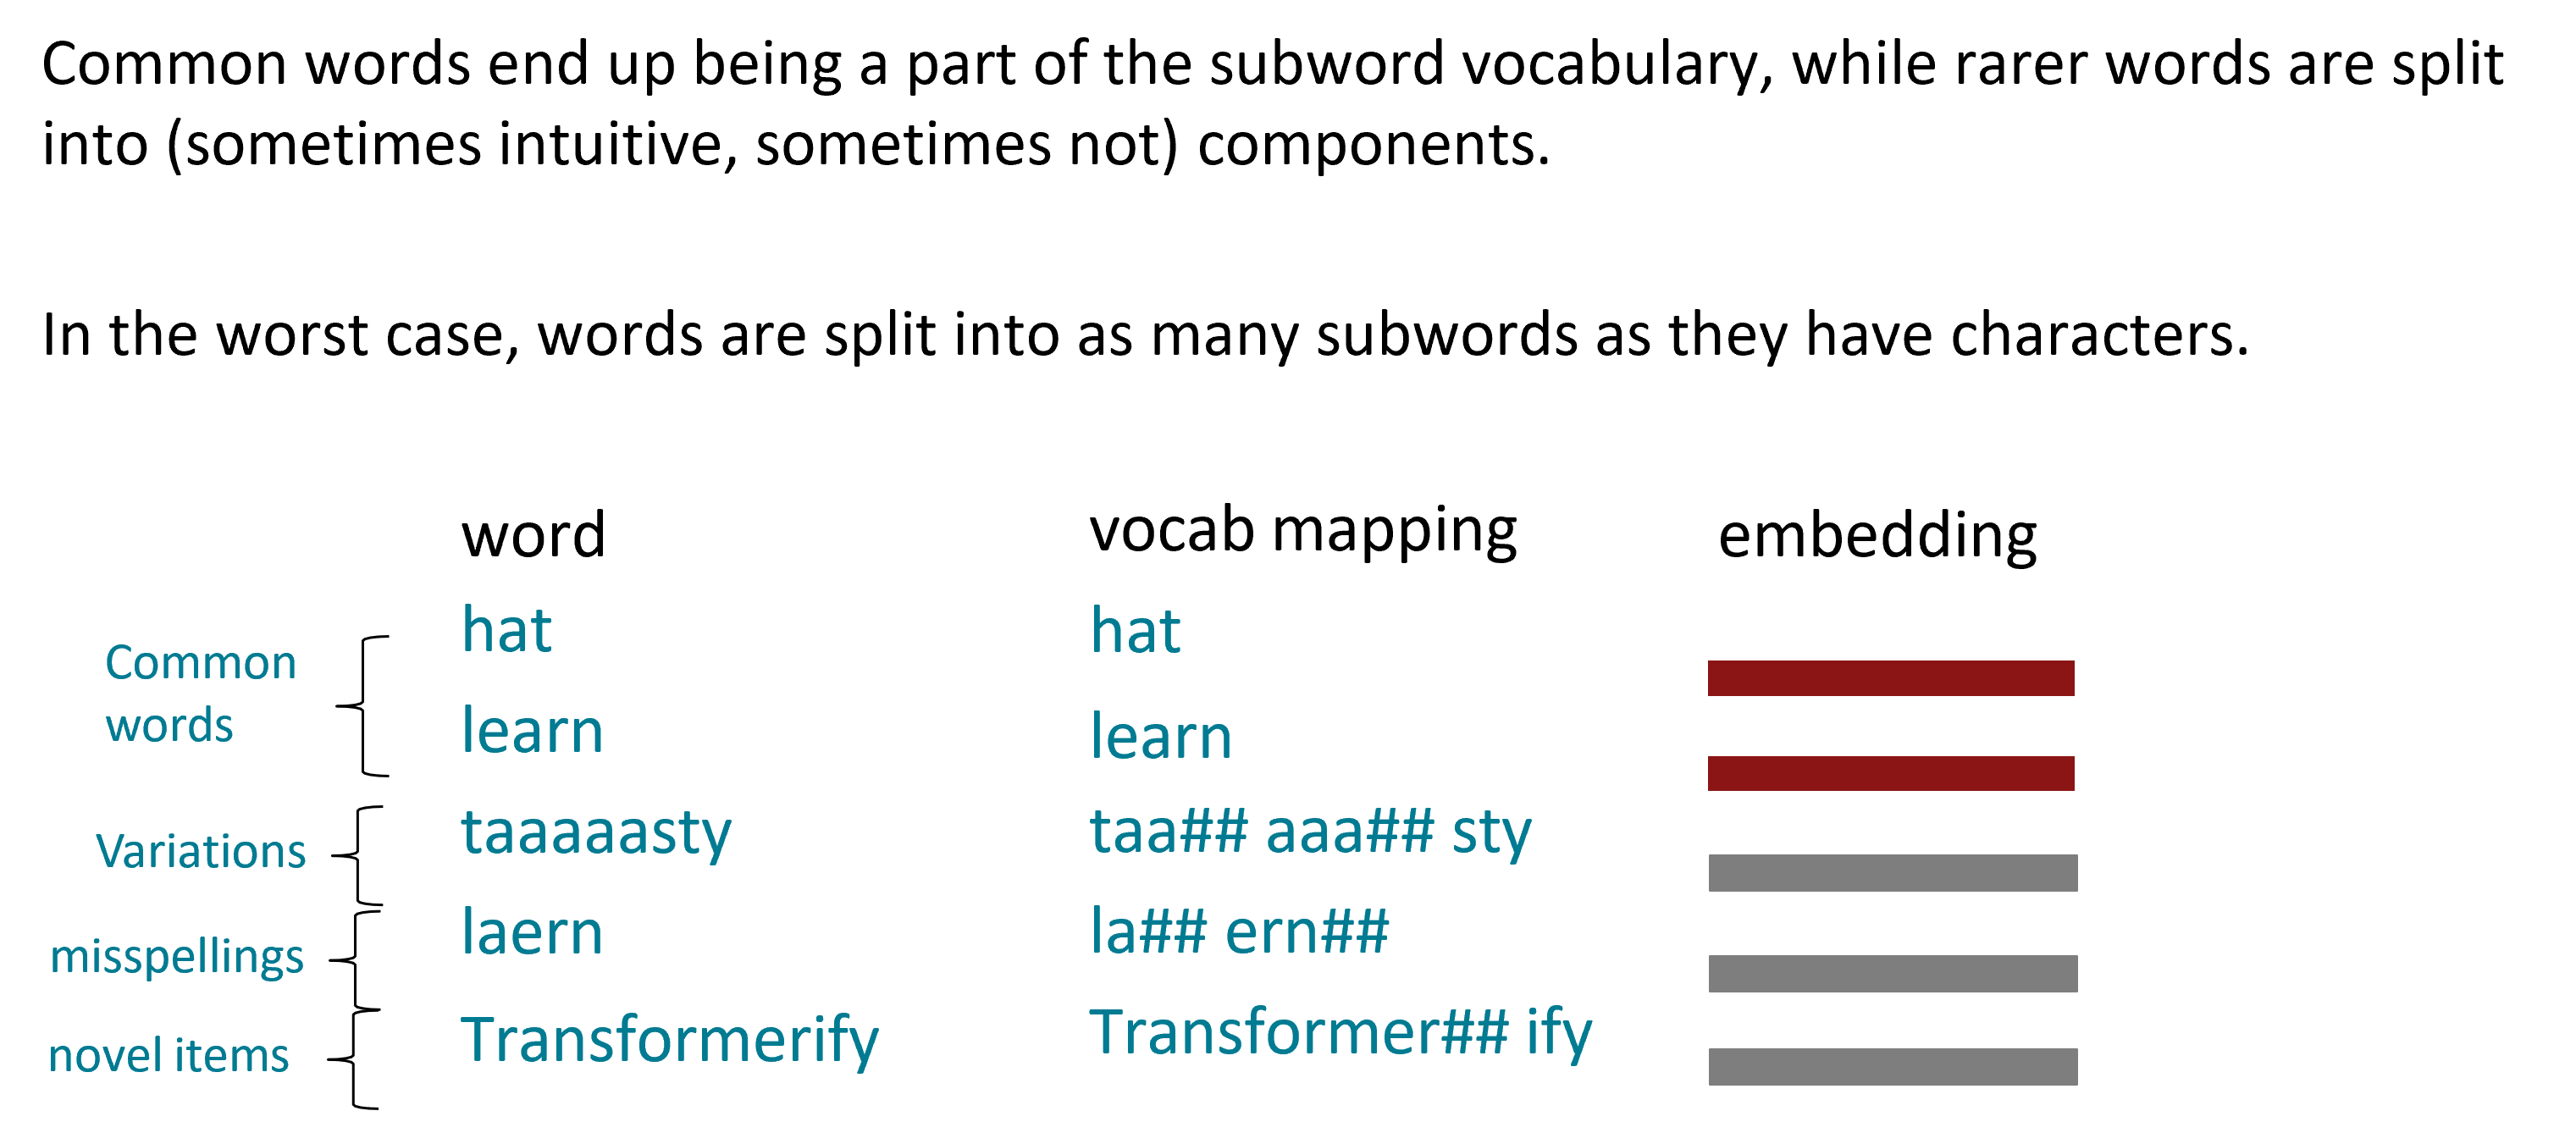
\includegraphics[width=\linewidth,keepaspectratio]{bert112}
			% \end{center}		
			
			% % {\tiny (Ref: John Hewitt)}

% \end{frame}

%%%%%%%%%%%%%%%%%%%%%%%%%%%%%%%%%%%%%%%%%%%%%%%%%%%%%%%%%%%%%%%%%%%%%%%%%%%%%%%%%%
\begin{frame}[fragile]\frametitle{}
\begin{center}
{\Large GPT}
\end{center}
\end{frame}


%%%%%%%%%%%%%%%%%%%%%%%%%%%%%%%%%%%%%%%%%%%%%%%%%%%%%%%%%%%
\begin{frame}[fragile]\frametitle{Generative Pretrained Transformer (GPT)}

[Radford et al., 2018]

2018’s GPT was a big success in pretraining a decoder!


      \begin{itemize}
			\item Transformer decoder with 12 layers.
			\item 768-dimensional hidden states, 3072-dimensional feed-forward hidden layers.
			\item Byte-pair encoding with 40,000 merges
			\item Trained on BooksCorpus: over 7000 unique books.
			\item Contains long spans of contiguous text, for learning long-distance dependencies.
			\item The acronym ``GPT'' never showed up in the original paper; it could stand for
			\item ``Generative PreTraining'' or ``Generative Pretrained Transformer''
			\end{itemize}

			
			% {\tiny (Ref: John Hewitt)}

\end{frame}

%%%%%%%%%%%%%%%%%%%%%%%%%%%%%%%%%%%%%%%%%%%%%%%%%%%%%%%%%%%
\begin{frame}[fragile]\frametitle{GPT}

			\begin{center}
			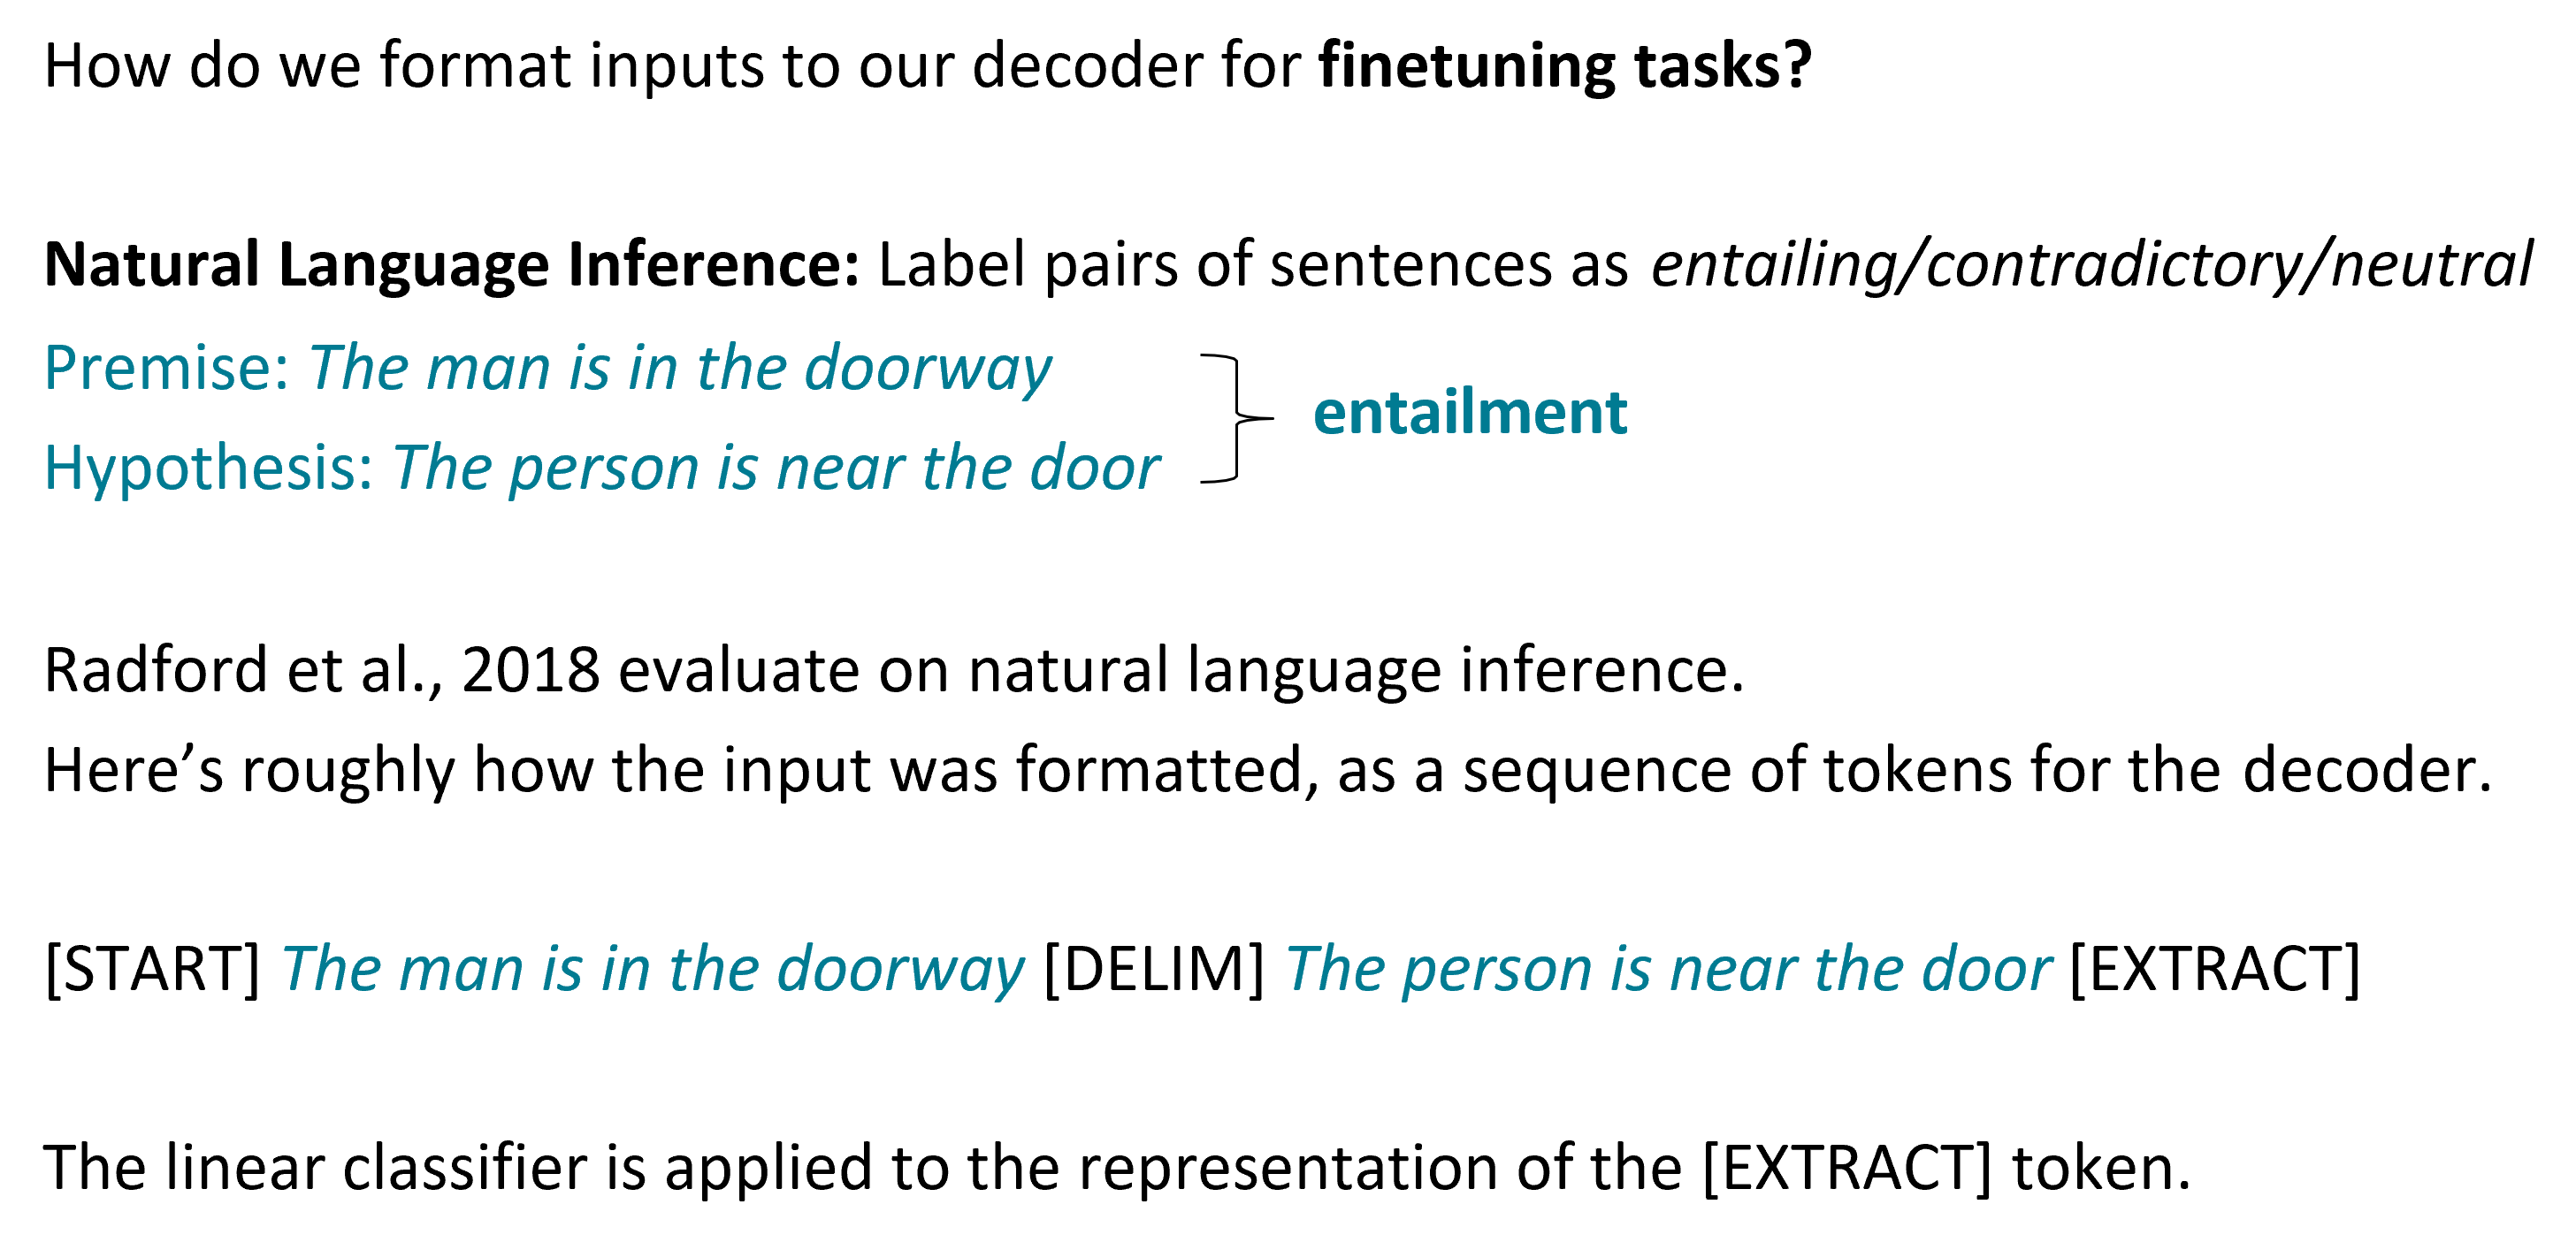
\includegraphics[width=\linewidth,keepaspectratio]{bert106}
			\end{center}		
			
			% {\tiny (Ref: John Hewitt)}

\end{frame}

%%%%%%%%%%%%%%%%%%%%%%%%%%%%%%%%%%%%%%%%%%%%%%%%%%%%%%%%%%%
\begin{frame}[fragile]\frametitle{GPT}

			\begin{center}
			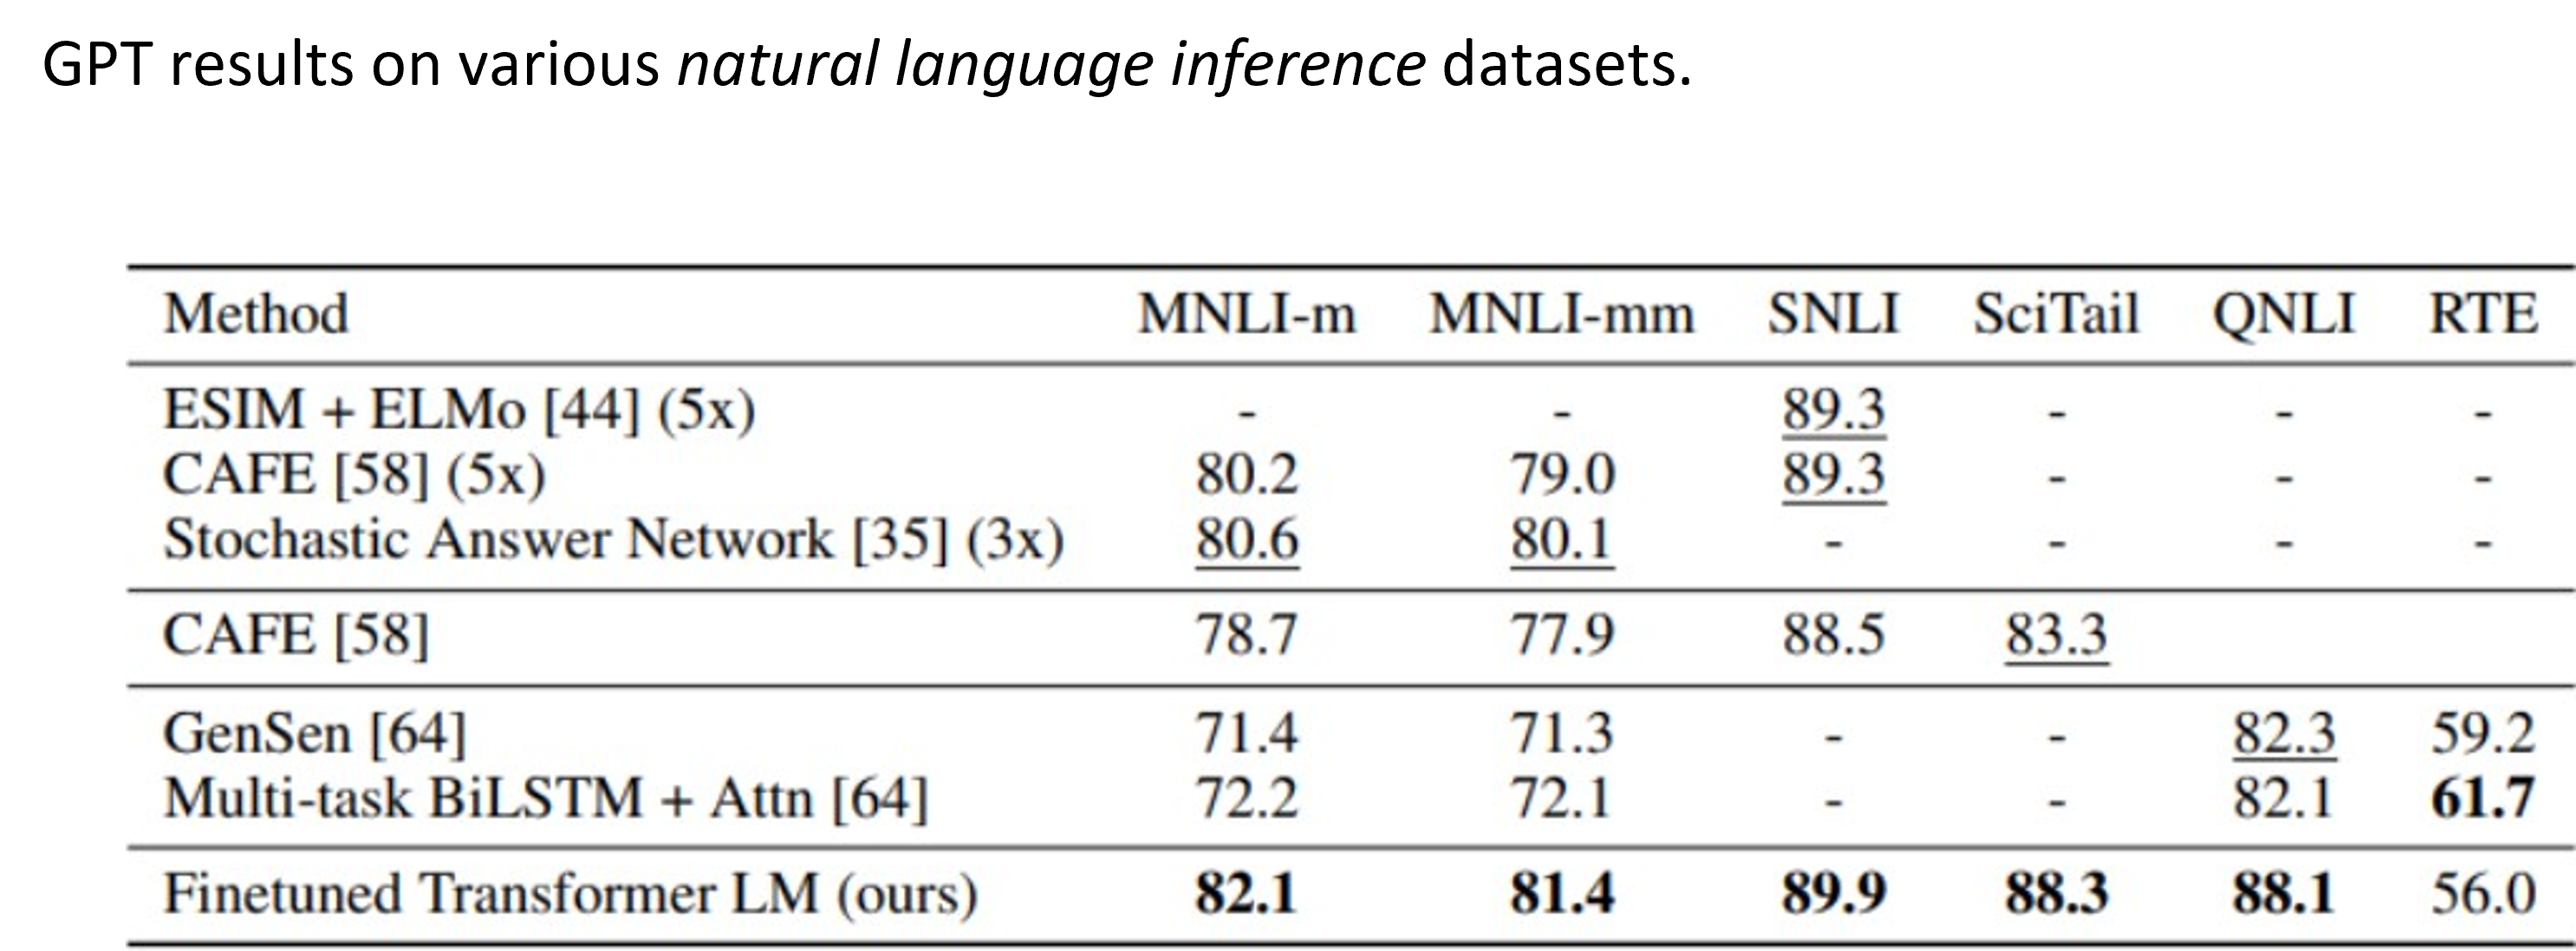
\includegraphics[width=\linewidth,keepaspectratio]{bert107}
			\end{center}		
			
			% {\tiny (Ref: John Hewitt)}

\end{frame}

%%%%%%%%%%%%%%%%%%%%%%%%%%%%%%%%%%%%%%%%%%%%%%%%%%%%%%%%%%%
\begin{frame}[fragile]\frametitle{GPT}

			\begin{center}
			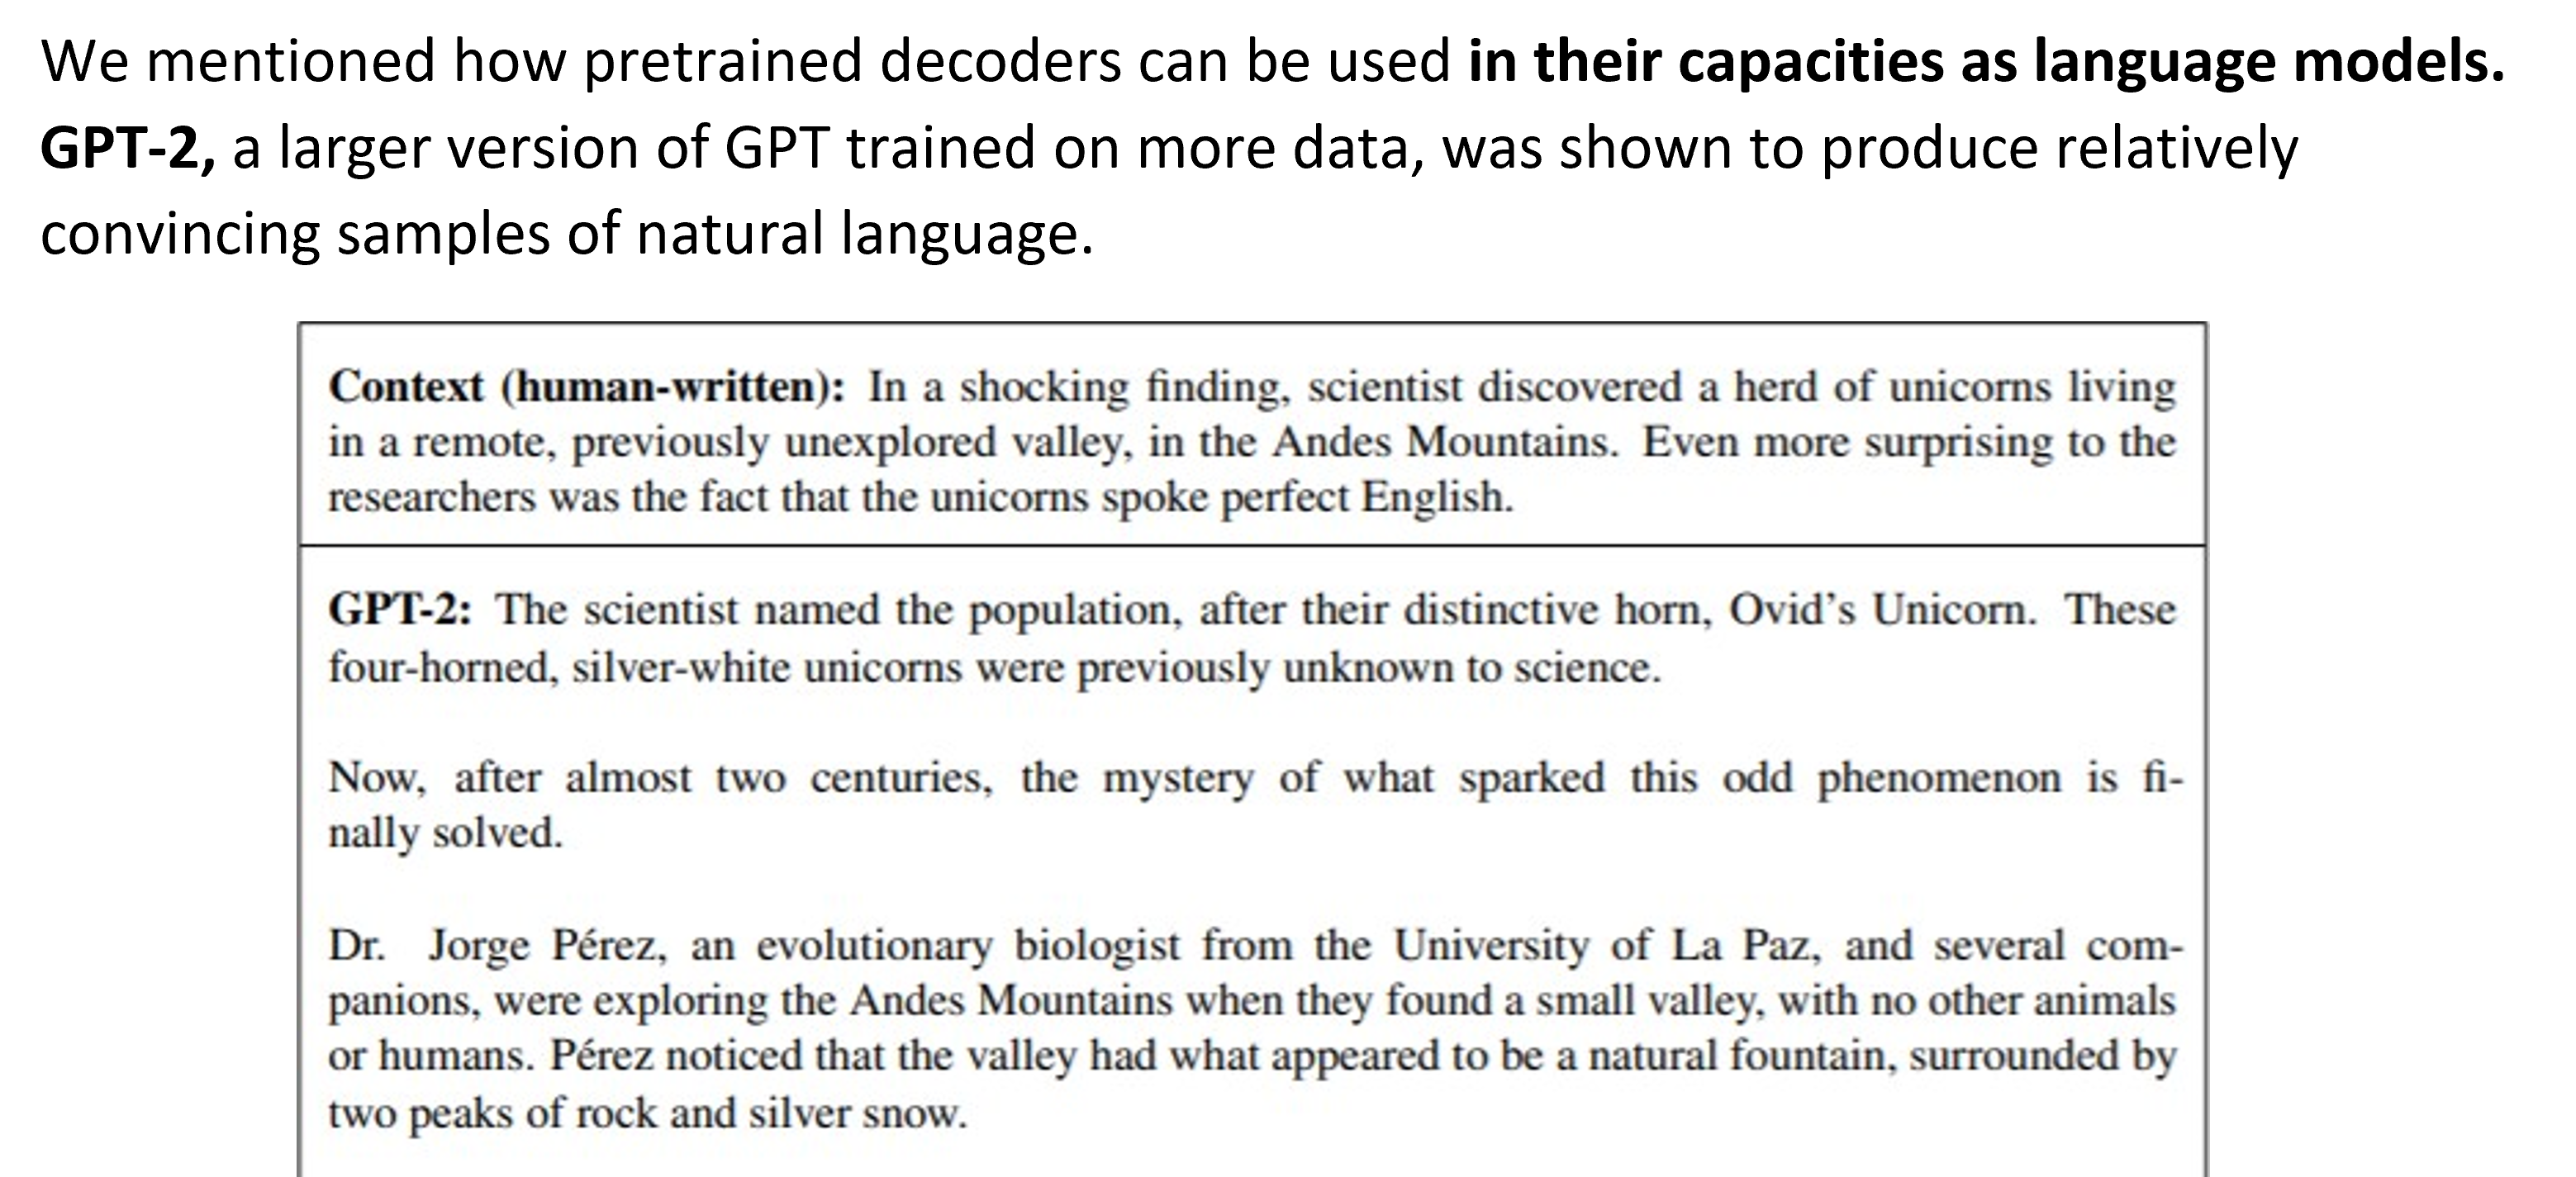
\includegraphics[width=\linewidth,keepaspectratio]{bert108}
			\end{center}		
			
			% {\tiny (Ref: John Hewitt)}

\end{frame}



%%%%%%%%%%%%%%%%%%%%%%%%%%%%%%%%%%%%%%%%%%%%%%%%%%%%%%%%%%%
\begin{frame}[fragile]\frametitle{GPT-3, in-context learning, very large models}


      \begin{itemize}
			\item So far, we’ve interacted with pretrained models in two ways:
			      \begin{itemize}
						\item Sample from the distributions they define (maybe providing a prompt)
						\item Fine-tune them on a task we care about, and take their predictions.
						\end{itemize}
			\item Very large language models seem to perform some kind of learning without gradient  steps simply from examples you provide within their contexts.
			\item GPT-3 is the canonical example of this. The largest T5 model had 11 billion parameters.
			\item GPT-3 has 175 billion parameters.

			\end{itemize}

			% {\tiny (Ref: John Hewitt)}

\end{frame}

%%%%%%%%%%%%%%%%%%%%%%%%%%%%%%%%%%%%%%%%%%%%%%%%%%%%%%%%%%%
\begin{frame}[fragile]\frametitle{GPT-3, in-context learning, very large models}


      \begin{itemize}
			\item Very large language models seem to perform some kind of learning without gradient  steps simply from examples you provide within their contexts.
			\item The in-context examples seem to specify the task to be performed, and the conditional  distribution mocks performing the task to a certain extent.
			\item Input (prefix within a single Transformer decoder context):
			\end{itemize}

			\begin{center}
			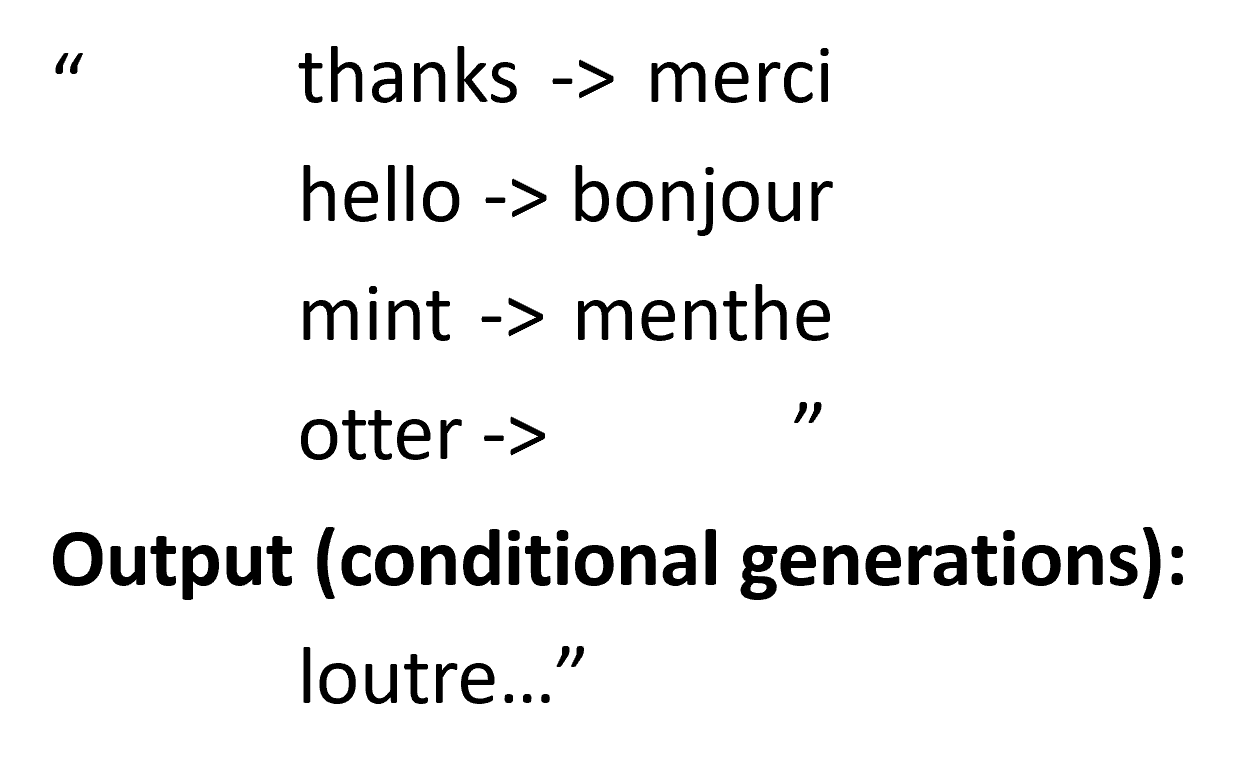
\includegraphics[width=0.4\linewidth,keepaspectratio]{bert102}
			\end{center}		
			
			% {\tiny (Ref: John Hewitt)}

\end{frame}

%%%%%%%%%%%%%%%%%%%%%%%%%%%%%%%%%%%%%%%%%%%%%%%%%%%%%%%%%%%
\begin{frame}[fragile]\frametitle{GPT-3, in-context learning, very large models}


			\begin{center}
			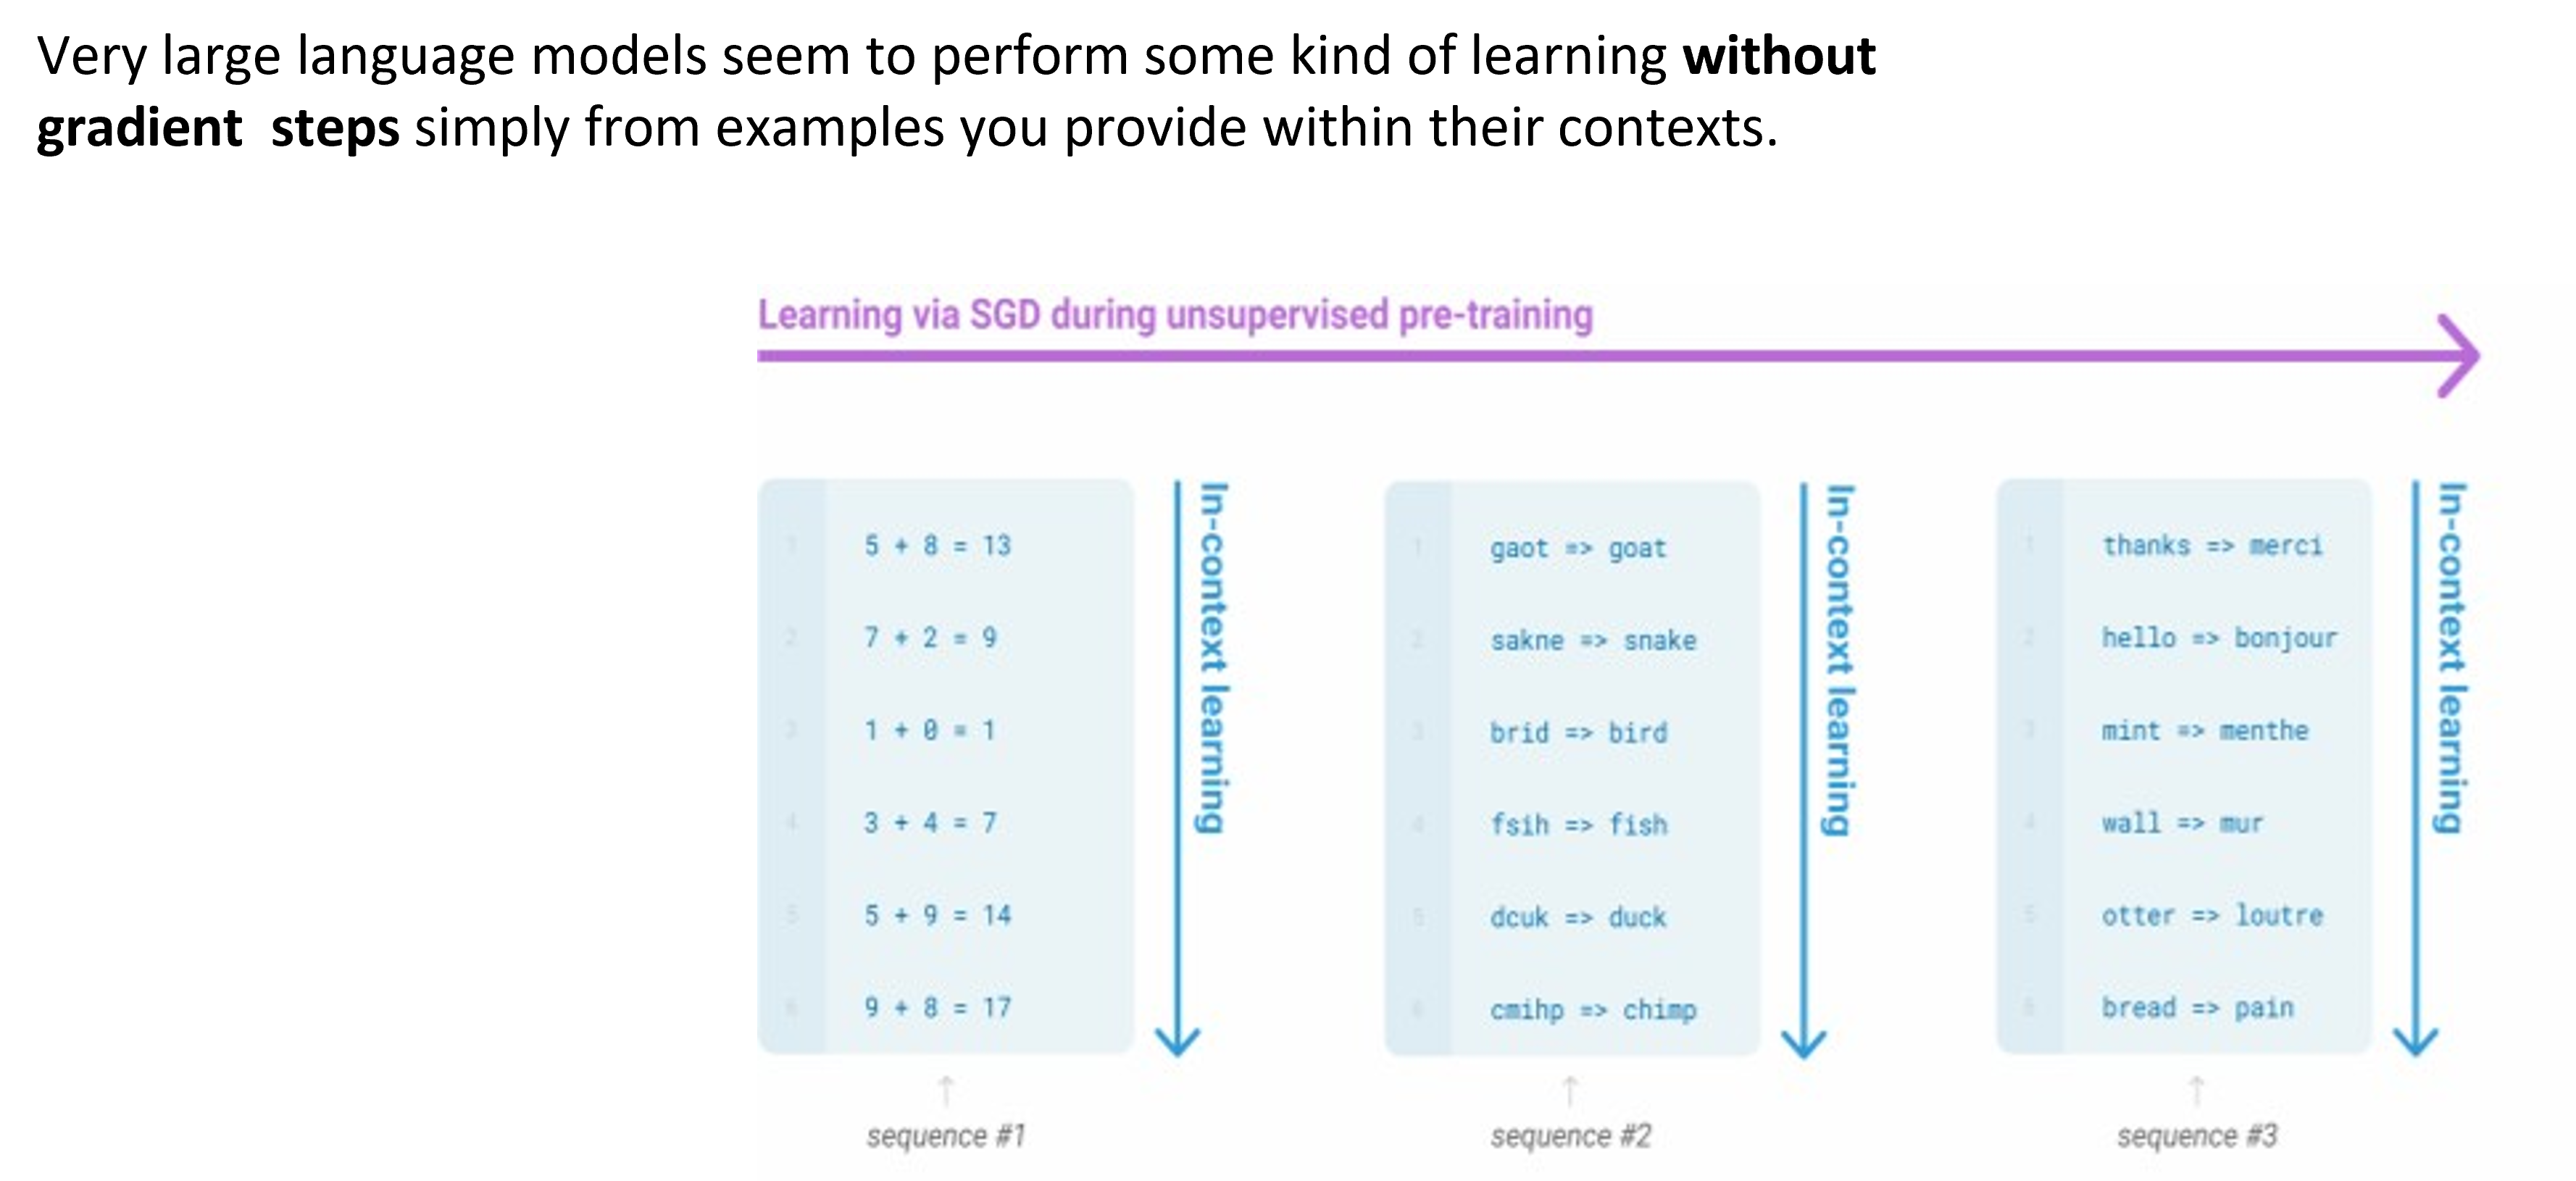
\includegraphics[width=\linewidth,keepaspectratio]{bert103}
			\end{center}		
			
			% {\tiny (Ref: John Hewitt)}

\end{frame}
